%% ═══════════════════════════════════════════════════════════════════════════
%% DATA — included via %% ═══════════════════════════════════════════════════════════════════════════
%% DATA — included via %% ═══════════════════════════════════════════════════════════════════════════
%% DATA — included via %% ═══════════════════════════════════════════════════════════════════════════
%% DATA — included via \input{data_section} from main.tex
%% ═══════════════════════════════════════════════════════════════════════════

\section{Data}\label{sec:data}

The data sources, sample construction, and feature definitions used throughout the thesis are described below. All data are at the monthly frequency. The stock-level sample spans January 1990 to November 2025, while the HMM regime model uses data from January 1990 onward (determined by the availability of stock-level data for computing cross-sectional return dispersion and relative market participation). The sample is split into a training period (pre-2011) used to estimate the HMM and cross-sectional models, and an out-of-sample test period (2011--2025) used exclusively for performance evaluation. Table~\ref{tab:sample_summary} provides an overview of the sample.

\begin{table}[H]
\centering
\begin{tabular}{l r r r}
\toprule
 & Train (1990--2010) & Test (2011--2025) & Full \\
\midrule
Unique stocks & 15{,}232 & 7{,}473 & 18{,}700 \\
Stock-month observations & 1{,}442{,}168 & 640{,}317 & 2{,}082{,}485 \\
Avg.\ stocks per month & 5{,}723 & 3{,}811 & 4{,}958 \\
Market-level months & 252 & 167 & 419 \\
\bottomrule
\end{tabular}
\caption{Sample summary.}
\label{tab:sample_summary}

\medskip
\small
\textbf{Notes:} The sample includes all ordinary common shares (CRSP share codes 10 and 11) listed on the NYSE, AMEX, or NASDAQ with a price above \$1. The decline in the average number of stocks in the test period reflects ongoing market consolidation and tighter listing standards.
\end{table}

\subsection{Data Sources}\label{sec:data_sources}

Three primary data sources are used:

\begin{itemize}
    \item \textbf{CRSP} (Center for Research in Security Prices, accessed via WRDS): Monthly stock-level returns, prices, shares outstanding, exchange codes, and share codes from the Monthly Stock File (\texttt{crsp.msf}). Daily market returns from the Daily Stock Index file (\texttt{crsp.dsi}) are used to compute the market drawdown feature. Delisting returns from \texttt{crsp.msedelist} are incorporated to avoid survivorship bias.
    \item \textbf{Compustat} (accessed via WRDS): Quarterly fundamental accounting data from \texttt{comp.fundq}, linked to CRSP via the CCM bridge table (\texttt{crsp.ccmxpf\_lnkhist}) using primary link types (LU, LC) with primary link indicators (P, C). Only observations where the fiscal quarter date falls within the active link window are retained. Variables include book equity (\texttt{ceqq}), total assets (\texttt{atq}), income before extraordinary items (\texttt{ibq}), revenue (\texttt{revtq}), cost of goods sold (\texttt{cogsq}), and debt (\texttt{dlttq}, \texttt{dlcq}).
    \item \textbf{FRED} (Federal Reserve Economic Data): Moody's BAA and AAA corporate bond yields, used to compute the credit spread (CS) that enters the final HMM specification (see Section~\ref{sec:feature_selection}). The CBOE Volatility Index (VIX) was also evaluated as a candidate but was not selected. The HMM sample begins in 1990, determined by the availability of stock-level data for computing cross-sectional return dispersion and relative market participation.
\end{itemize}

\subsection{Stock Universe and Filtering}\label{sec:stock_universe}

The stock-level sample includes all ordinary common shares (CRSP share codes 10 and 11) listed on the NYSE, AMEX, or NASDAQ (exchange codes 1, 2, and 3). This excludes American Depositary Receipts (ADRs), Real Estate Investment Trusts (REITs), closed-end funds, and other non-standard securities. A minimum price filter of \$1 is applied to remove penny stocks, whose extreme percentage returns and low liquidity would distort momentum signals.\footnote{This filter is standard in the momentum literature; see, e.g., \citet{JegadeeshTitman2001}. Stocks priced below \$1 can exhibit percentage returns of hundreds of percent from small absolute price changes, contaminating momentum signals.}

\paragraph{Delisting adjustment}
Following \citet{Shumway2001}, delisting returns are incorporated to prevent survivorship bias. When a stock is delisted, its actual delisting return is used if available; for performance-related delistings (CRSP codes 500--584) with missing returns, $-30\%$ is imputed.

\subsection{HMM Regime Features}\label{sec:hmm_features}

The Hidden Markov Model takes as input four macrofinancial stress indicators, selected through the systematic procedure described in Section~\ref{sec:feature_selection}. All four indicators are \textbf{observable in real time} at the end of each month.\footnote{``Real time'' means that each feature can be computed from data available on the last trading day of the month, with no reporting lag or subsequent revision. This is in contrast to macroeconomic indicators such as GDP, which are released with a delay and revised multiple times.} This real-time availability is essential: because the filtered regime probability $\pi_t^{\text{filter}}$ is used as a trading signal, any feature with a reporting lag would introduce look-ahead bias. Indicators such as GDP growth, which is published with a delay of approximately one month and subject to subsequent revisions, are therefore excluded despite their economic relevance.

The four features are:

\begin{enumerate}
    \item \textbf{DD (Drawdown):} The percentage decline of the cumulative market price index from its rolling 12-month peak:
    \begin{equation}
        DD_t = \frac{P_t - \max(P_{t-11}, \dots, P_t)}{\max(P_{t-11}, \dots, P_t)},
    \end{equation}
    where $P_t = 100 \times \prod_{\tau=1}^{t}(1 + r_\tau^{\text{mkt}})$ is the cumulative value-weighted market return index. DD is always non-positive and captures the magnitude of an ongoing downturn. \citet{DanielMoskowitz2016} show that the conditional volatility of momentum strategies is strongly related to past market declines, as drawdowns trigger forced selling and margin calls that reverse momentum profits. DD directly measures this mechanism and, as shown in Section~\ref{sec:ablation_results}, is the single most informative HMM input feature for downstream portfolio performance.

    \item \textbf{DISP (Return Dispersion):} The log cross-sectional standard deviation of individual stock returns within each month:
    \begin{equation}
        DISP_t = \log\!\left(\text{std}_s(r_{s,t})\right),
    \end{equation}
    where $\text{std}_s$ denotes the standard deviation computed across all stocks $s$ in the universe in month~$t$. Return dispersion captures cross-sectional \emph{disagreement} among individual stocks. During stress, consensus breaks down and dispersion spikes, signalling changes in the correlation structure that affect momentum profits.

    \item \textbf{REL\_N (Relative Market Participation):} The log ratio of the number of actively traded stocks in month~$t$ to its trailing 12-month moving average:
    \begin{equation}
        REL\_N_t = \log\!\left(\frac{N_t}{\frac{1}{12}\sum_{\ell=1}^{12} N_{t-\ell}}\right),
    \end{equation}
    where $N_t$ is the number of stocks with valid return observations in month~$t$. REL\_N is close to zero in normal times but turns negative during crises when stocks delist, halt trading, or are acquired at elevated rates. For example, during the 2008 financial crisis, a wave of delistings and trading halts caused $N_t$ to drop sharply relative to its trailing average. This captures structural market damage that the other three features do not measure.

    \item \textbf{CS (Credit Spread):} The difference between Moody's BAA and AAA corporate bond yields:
    \begin{equation}
        CS_t = Y_t^{\text{BAA}} - Y_t^{\text{AAA}}.
    \end{equation}
    The credit spread widens when investors demand higher compensation for default risk, making it a leading indicator of financial stress that is distinct from the equity-based features above. Unlike DD, DISP, and REL\_N, which are derived entirely from equity market data, CS provides an independent signal from the corporate bond market. This cross-market information helps the HMM distinguish genuine stress episodes from equity-specific turbulence.
\end{enumerate}

\begin{figure}[H]
    \centering
    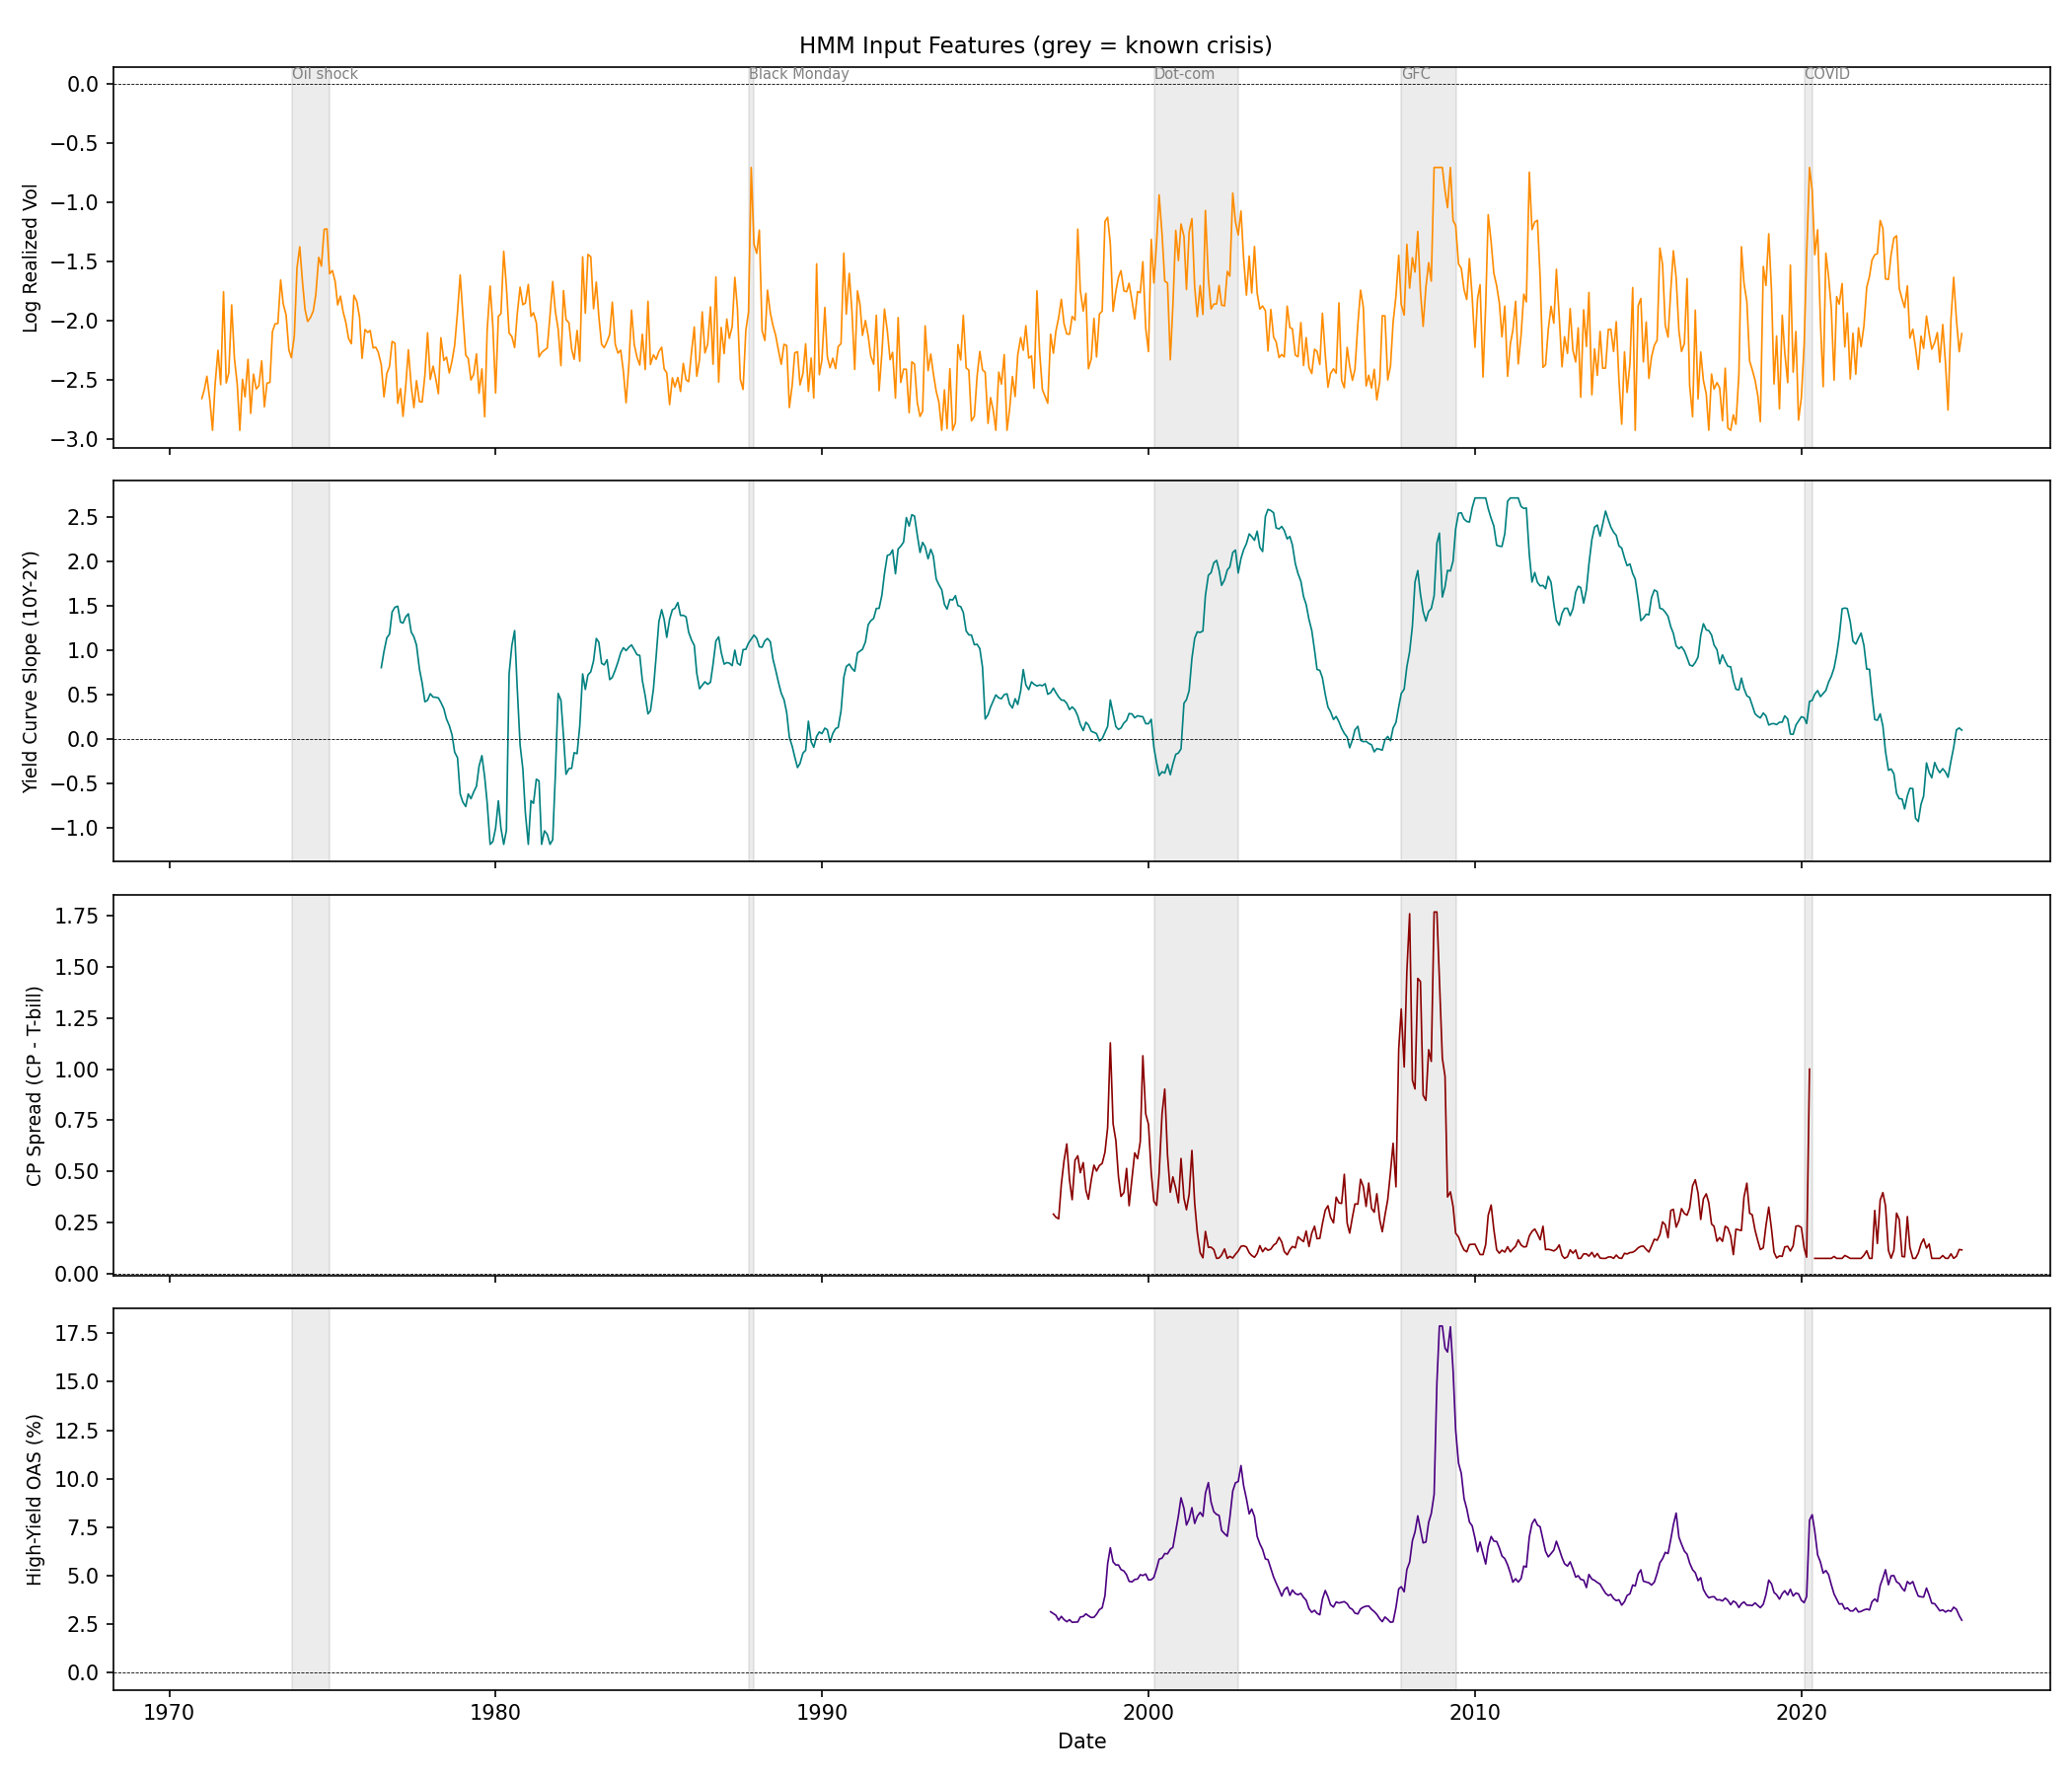
\includegraphics[width=\textwidth]{features_hmm.png}
    \caption{Time series of the four HMM input features (DD, DISP, REL\_N, CS), standardised using training-sample statistics. Shaded regions indicate NBER recession periods. All four features respond during the dot-com bust (2000--2002) and the global financial crisis (2007--2009), but with distinct dynamics reflecting their complementary stress dimensions.}
    \label{fig:features_hmm}
\end{figure}

\paragraph{Why these four features together}
The four selected indicators span complementary dimensions of market stress: DD captures the depth of equity market declines, DISP and REL\_N describe cross-sectional behaviour (stock disagreement and structural attrition), and CS captures corporate credit conditions. The feature selection procedure in Section~\ref{sec:feature_selection} confirms that this combination, drawn from a broader candidate pool of nine indicators including volatility and options market indicators, produces the most robust regime signal for the downstream momentum strategies.

\paragraph{Preprocessing}
All four features are winsorised at the 1st and 99th percentiles to limit the influence of extreme outliers.\footnote{Winsorisation replaces observations below the $p$-th percentile with the $p$-th percentile value, and observations above the $(1-p)$-th percentile with the $(1-p)$-th percentile value. Unlike trimming, which discards extreme observations entirely, winsorisation retains all data points while bounding their magnitude. This is particularly important for the HMM emission densities, which assume multivariate normality and can be distorted by heavy-tailed outliers.} The winsorisation bounds are computed on the training sample (1990--2010) and applied unchanged to the test sample, preventing information leakage. After winsorisation, each feature is standardised to zero mean and unit variance using training-sample statistics:
\begin{equation}
    z_{j,t} = \frac{x_{j,t} - \bar{x}_j^{\text{train}}}{\sigma_j^{\text{train}}}.
\end{equation}
Standardisation ensures that all features contribute equally to the HMM's Gaussian emission densities, so that the regime classification is not dominated by whichever feature has the largest raw scale.

\subsection{HMM Feature Selection}\label{sec:feature_selection}

The choice of HMM input features has a substantial impact on regime classification quality and, ultimately, on portfolio performance. This thesis selects features through a systematic three-pass pipeline that progressively filters candidates and increases computational rigor at each stage.

\paragraph{Candidate pool}
Nine monthly macrofinancial indicators, all available from 1990 onward, are considered as HMM inputs. These span three broad categories of market stress:
\begin{itemize}
    \item \emph{Equity market:} market drawdown (DD), realised volatility (VOL), cross-sectional return dispersion (DISP), relative market participation (REL\_N), advance-decline ratio (ADR), and cross-sectional return skewness (SKEW).
    \item \emph{Credit and macro:} BAA--AAA credit spread (CS), log VIX (LVIX), and the 10-year minus 2-year Treasury term spread (TERM).
\end{itemize}
All candidates are observable in real time at the end of each month. Two additional credit indicators (the commercial paper spread and the high-yield option-adjusted spread) are excluded because their data begins in the mid-1990s, providing insufficient training coverage for the 1990--2010 estimation window. All features are standardised to $z$-scores using training-period means and standard deviations, applied unchanged to the test period.

\paragraph{Pass~1: Quality screen}
Because market drawdown (DD) is the most economically direct measure of equity stress and consistently emerges as the dominant regime-identifying feature, it is required in every combination. The remaining eight candidates are combined with DD in groups of 1 to 3 additional features, yielding $1 + \binom{8}{1} + \binom{8}{2} + \binom{8}{3} = 93$ combinations spanning 1- to 4-feature HMMs. Each combination is estimated with a single Gibbs sampler seed (2{,}000 iterations, 500 burn-in). A combination passes the quality screen if it satisfies five criteria: (i)~minimum effective sample size (ESS) across all posterior mean parameters exceeds 50; (ii)~at least $\min(2, D)$ features exhibit statistically significant regime separation (95\% credible interval excluding zero); (iii)~the average filtered panic probability during the GFC (October 2007 to June 2009) exceeds 0.5 and during COVID (February to May 2020) exceeds 0.5; (iv)~the average panic probability during non-crisis reference periods (January 2003 to December 2006, and January 2013 to December 2019) remains below 0.4; and (v)~the Dot-com crash (March 2000 to October 2002) average exceeds 0.3. Panic state identification uses the same sign-correction method as the main HMM (Section~\ref{sec:gibbs}): the direction of each feature during known crises is determined empirically, and the state with the higher sign-corrected posterior mean is labelled as panic.

\paragraph{Pass~2: Portfolio ranking}
Surviving combinations are evaluated through the full cross-sectional pipeline. The filtered probability $\pi_t^{\text{filter}}$ is averaged across 5 HMM seeds to reduce MCMC noise. XGBoost predictions are averaged across 10 seeds to stabilise stock rankings. To maintain a fair comparison with the exposure-scaling approach of \citet{DanielMoskowitz2016}, portfolios use momentum and $\pi_t^{\text{filter}}$ only (no fundamental features) and are constructed as long-short with 10 basis points one-way costs applied to both legs. Combinations are ranked by out-of-sample Sharpe ratio. The top 10 advance to Pass~3.

\paragraph{Pass~3: Definitive validation}
The final pass increases seed counts to 10 HMM seeds and 20 XGBoost seeds. For each surviving combination, four tests are conducted:
\begin{enumerate}
    \item \emph{Ensemble Sharpe ratio} from the averaged predictions, representing the strategy's performance under heavy seed averaging.
    \item \emph{Sub-period consistency}: Sharpe ratios for 2011--2015, 2016--2020, and 2021--2025, verifying that performance is not driven by a single sub-period.
    \item \emph{Stability test}: 20 independent experiments, each using a random partition of 3 HMM seeds and 1 XGBoost seed drawn from a pool of 20, to assess sensitivity to the specific seed combination. Combinations are classified as stable ($\sigma < 0.10$), moderate ($0.10 \leq \sigma < 0.15$), or unstable ($\sigma \geq 0.15$).
    \item \emph{Leave-one-year-out}: each test-period year is dropped in turn to verify that no single year drives the result.
\end{enumerate}

\paragraph{Feature count comparison}
The pipeline evaluates combinations of 1 to 4 features to determine the optimal model complexity. Table~\ref{tab:feature_selection} reports the top combination at each feature count. Four features (DD+DISP+REL\_N+CS) achieves the highest stability mean (0.804) with the lowest standard deviation (0.082), indicating that the additional features reduce seed sensitivity without introducing overfitting. This combination is confirmed by a heavy variance test: 10 independent runs, each using 20 fresh HMM seeds (seeds 1--200) and 50 XGBoost seeds, produce a mean Sharpe of 0.804 with standard deviation 0.082.

\input{tables/table_feature_selection}

\paragraph{Ablation analysis}
Single-feature and leave-one-out experiments isolate each feature's marginal contribution to the selected combination. DD alone achieves a Sharpe of 0.66, confirming its role as the dominant stress indicator. In the leave-one-out analysis, removing DD or REL\_N causes the largest performance drops ($-0.46$ and $-0.54$, respectively), while DISP and CS each contribute less than 0.01 marginally. Despite their small marginal contributions, DISP and CS improve the stability of the regime signal by providing independent information from different market segments (cross-sectional disagreement and corporate credit stress, respectively). The full ablation results are reported in Section~\ref{sec:ablation_results}.

\paragraph{Summary}
The selected feature set, DD+DISP+REL\_N+CS, captures market stress through three complementary dimensions: the depth of equity market declines (DD), cross-sectional stock disagreement (DISP) and structural market attrition (REL\_N), and corporate credit conditions (CS). All four features are available from January 1990, providing 241 training months that include both the dot-com crash and the global financial crisis. The final $\pi_t^{\text{filter}}$ used in all subsequent analyses is averaged across 200 HMM seeds and passes all three validation checks (regime separation, crisis alignment, and MCMC convergence).

\subsection{Cross-Sectional Features}\label{sec:cs_features}

The cross-sectional models use three groups of features to rank stocks each month: momentum signals, the filtered panic probability $\pi_t^{\text{filter}}$, and fundamental characteristics.

\paragraph{Momentum lookbacks}
Twelve trailing momentum signals are computed for each stock, corresponding to lookback horizons of 1 to 12 months:
\begin{equation}
    \text{mom}_{k,t}^s = \prod_{\ell=1}^{k}(1 + r_{t-\ell}^s) - 1, \qquad k = 1, \dots, 12,
\end{equation}
where $r_{t-\ell}^s$ is the adjusted return of stock $s$ in month $t - \ell$. Note that the current month's return is excluded from all lookbacks to avoid mechanical correlation with the forward return being predicted. Including all twelve horizons rather than a single lookback (e.g., the standard 12-month momentum of \citet{JegadeeshTitman1993}) allows the models to learn which horizons are most informative in each regime. As shown in Section~\ref{sec:ic_analysis}, intermediate-term lookbacks (8--11 months) dominate in calm markets, while 1-month momentum becomes important during panic due to short-term reversal dynamics.

\paragraph{Regime signal}
The filtered panic probability $\pi_t^{\text{filter}}$ from the HMM enters as a single feature. Because it varies only at the monthly market level (every stock in the same month receives the same value), it functions as a conditioning variable rather than a stock-level predictor. Its role in the cross-sectional models is discussed in Section~\ref{sec:ic_analysis}.

\paragraph{Fundamental characteristics}
Seven firm-level characteristics are computed from Compustat quarterly data. These variables are drawn from the established asset pricing literature: book-to-market and size are the original \citet{FamaFrench2015} factors, gross profitability follows \citet{NovyMarx2013}, and the remaining variables (leverage, asset growth, return on equity, earnings growth) capture investment and quality dimensions that have been shown to predict cross-sectional returns. Their role in the models is not to generate additional returns but to act as a quality screen that compresses portfolio volatility (see Section~\ref{sec:performance_results}).

\begin{itemize}
    \item \textbf{Book-to-market (bm):} Book equity divided by market equity, $\text{ceqq} / ME$. Captures the value premium.
    \item \textbf{Return on equity (roe):} Income before extraordinary items divided by book equity, $\text{ibq} / \text{ceqq}$. Measures profitability.
    \item \textbf{Gross profitability:} Revenue minus cost of goods sold, scaled by total assets, $(\text{revtq} - \text{cogsq}) / \text{atq}$. Follows the profitability factor of \citet{NovyMarx2013}.
    \item \textbf{Asset growth:} Year-over-year growth in total assets, $\text{atq}_t / \text{atq}_{t-4} - 1$. Firms with high asset growth tend to have lower future returns.
    \item \textbf{Leverage:} Total debt divided by total assets, $(\text{dlttq} + \text{dlcq}) / \text{atq}$. Highly leveraged firms are more vulnerable to financial distress.
    \item \textbf{Earnings growth:} Year-over-year growth in earnings, computed as $\text{sign}(g) \cdot \log(1 + |g|)$ where $g = \text{ibq}_t / \text{ibq}_{t-4} - 1$. The signed-log transformation handles the fat-tailed distribution of earnings changes.
    \item \textbf{Log market equity:} The natural logarithm of market capitalisation (price times shares outstanding), lagged one month. Controls for the size effect.
\end{itemize}

Market equity is computed as the absolute value of the end-of-month stock price multiplied by shares outstanding from CRSP. The absolute value handles cases where CRSP reports the bid-ask midpoint as a negative price.

All fundamental variables are lagged by four months relative to the fiscal quarter end to ensure that accounting data would have been publicly available at the time of portfolio formation, consistent with the standard approach in the empirical asset pricing literature. This lag accounts for the SEC filing deadline and prevents look-ahead bias. Each month, the most recent available quarter's fundamentals are assigned to each stock using a backward merge, so that no future accounting information is used. Fundamentals are winsorised at the 1st and 99th percentiles (5th and 95th for asset growth, which has a fatter right tail), with bounds computed on the training sample only.

\paragraph{Missing data handling}
Not all stocks have complete fundamental coverage in every month. Missing rates range from approximately 7\% (return on equity, leverage) to 17\% (gross profitability). For the logistic regression model, which cannot handle missing values, fundamentals are imputed at the training-sample median prior to standardisation. For XGBoost, which natively handles missing values by learning optimal split directions for absent features, no imputation is applied. In both cases, stocks are only excluded if core features (momentum lookbacks or the regime signal) are missing.

\subsection{Train--Test Split and Information Leakage Prevention}\label{sec:split}

The sample is divided at December 2010. The HMM start date of January 1990 is determined by the availability of sufficient stock-level data for computing cross-sectional return dispersion, and the split point is chosen so that the training period contains at least two full market cycles, including the dot-com crash (2000--2002) and the global financial crisis (2007--2009), giving the HMM sufficient exposure to both calm and panic regimes. The training period is used for all model estimation: HMM Gibbs sampling, logistic regression fitting, and XGBoost training. The test period (January 2011 to November 2025, 167 months) is reserved exclusively for out-of-sample evaluation; no model parameters are re-estimated or updated during this period.

Several safeguards prevent information leakage from the test period into model training:
\begin{itemize}
    \item Winsorisation bounds and standardisation statistics (means, standard deviations) are computed on the training sample and applied unchanged to the test sample.
    \item The HMM posterior mean parameters (regime means $\boldsymbol{\mu}_k$, covariances $\boldsymbol{\Sigma}_k$, and transition matrix $\mathbf{P}$) are estimated on the training period and frozen. During the test period, only the forward-filtering recursion is run using the fixed parameters, producing the causal signal $\pi_t^{\text{filter}}$ without any parameter updating.
    \item The cross-sectional models are trained once on the training sample and applied without retraining to the test sample.
    \item NYSE breakpoints for portfolio decile assignment are computed each month using only NYSE-listed stocks in that month, which is observable in real time.
\end{itemize}

A single fixed split is standard in the literature that this thesis builds on \citep[e.g.,][]{GHM2023} and is appropriate given the computational cost of re-estimating the Bayesian HMM via Gibbs sampling. Alternative train/test splits (Appendix~\ref{app:alt_splits}) confirm that both M1 and M2 produce positive Sharpe ratios across all splits tested, though the baseline split yields the strongest M1 performance. The 14-year out-of-sample test period and the statistical significance tests reported in Section~\ref{sec:performance_results} further mitigate concerns about split dependence.
 from main.tex
%% ═══════════════════════════════════════════════════════════════════════════

\section{Data}\label{sec:data}

The data sources, sample construction, and feature definitions used throughout the thesis are described below. All data are at the monthly frequency. The stock-level sample spans January 1990 to November 2025, while the HMM regime model uses data from January 1990 onward (determined by the availability of stock-level data for computing cross-sectional return dispersion and relative market participation). The sample is split into a training period (pre-2011) used to estimate the HMM and cross-sectional models, and an out-of-sample test period (2011--2025) used exclusively for performance evaluation. Table~\ref{tab:sample_summary} provides an overview of the sample.

\begin{table}[H]
\centering
\begin{tabular}{l r r r}
\toprule
 & Train (1990--2010) & Test (2011--2025) & Full \\
\midrule
Unique stocks & 15{,}232 & 7{,}473 & 18{,}700 \\
Stock-month observations & 1{,}442{,}168 & 640{,}317 & 2{,}082{,}485 \\
Avg.\ stocks per month & 5{,}723 & 3{,}811 & 4{,}958 \\
Market-level months & 252 & 167 & 419 \\
\bottomrule
\end{tabular}
\caption{Sample summary.}
\label{tab:sample_summary}

\medskip
\small
\textbf{Notes:} The sample includes all ordinary common shares (CRSP share codes 10 and 11) listed on the NYSE, AMEX, or NASDAQ with a price above \$1. The decline in the average number of stocks in the test period reflects ongoing market consolidation and tighter listing standards.
\end{table}

\subsection{Data Sources}\label{sec:data_sources}

Three primary data sources are used:

\begin{itemize}
    \item \textbf{CRSP} (Center for Research in Security Prices, accessed via WRDS): Monthly stock-level returns, prices, shares outstanding, exchange codes, and share codes from the Monthly Stock File (\texttt{crsp.msf}). Daily market returns from the Daily Stock Index file (\texttt{crsp.dsi}) are used to compute the market drawdown feature. Delisting returns from \texttt{crsp.msedelist} are incorporated to avoid survivorship bias.
    \item \textbf{Compustat} (accessed via WRDS): Quarterly fundamental accounting data from \texttt{comp.fundq}, linked to CRSP via the CCM bridge table (\texttt{crsp.ccmxpf\_lnkhist}) using primary link types (LU, LC) with primary link indicators (P, C). Only observations where the fiscal quarter date falls within the active link window are retained. Variables include book equity (\texttt{ceqq}), total assets (\texttt{atq}), income before extraordinary items (\texttt{ibq}), revenue (\texttt{revtq}), cost of goods sold (\texttt{cogsq}), and debt (\texttt{dlttq}, \texttt{dlcq}).
    \item \textbf{FRED} (Federal Reserve Economic Data): Moody's BAA and AAA corporate bond yields, used to compute the credit spread (CS) that enters the final HMM specification (see Section~\ref{sec:feature_selection}). The CBOE Volatility Index (VIX) was also evaluated as a candidate but was not selected. The HMM sample begins in 1990, determined by the availability of stock-level data for computing cross-sectional return dispersion and relative market participation.
\end{itemize}

\subsection{Stock Universe and Filtering}\label{sec:stock_universe}

The stock-level sample includes all ordinary common shares (CRSP share codes 10 and 11) listed on the NYSE, AMEX, or NASDAQ (exchange codes 1, 2, and 3). This excludes American Depositary Receipts (ADRs), Real Estate Investment Trusts (REITs), closed-end funds, and other non-standard securities. A minimum price filter of \$1 is applied to remove penny stocks, whose extreme percentage returns and low liquidity would distort momentum signals.\footnote{This filter is standard in the momentum literature; see, e.g., \citet{JegadeeshTitman2001}. Stocks priced below \$1 can exhibit percentage returns of hundreds of percent from small absolute price changes, contaminating momentum signals.}

\paragraph{Delisting adjustment}
Following \citet{Shumway2001}, delisting returns are incorporated to prevent survivorship bias. When a stock is delisted, its actual delisting return is used if available; for performance-related delistings (CRSP codes 500--584) with missing returns, $-30\%$ is imputed.

\subsection{HMM Regime Features}\label{sec:hmm_features}

The Hidden Markov Model takes as input four macrofinancial stress indicators, selected through the systematic procedure described in Section~\ref{sec:feature_selection}. All four indicators are \textbf{observable in real time} at the end of each month.\footnote{``Real time'' means that each feature can be computed from data available on the last trading day of the month, with no reporting lag or subsequent revision. This is in contrast to macroeconomic indicators such as GDP, which are released with a delay and revised multiple times.} This real-time availability is essential: because the filtered regime probability $\pi_t^{\text{filter}}$ is used as a trading signal, any feature with a reporting lag would introduce look-ahead bias. Indicators such as GDP growth, which is published with a delay of approximately one month and subject to subsequent revisions, are therefore excluded despite their economic relevance.

The four features are:

\begin{enumerate}
    \item \textbf{DD (Drawdown):} The percentage decline of the cumulative market price index from its rolling 12-month peak:
    \begin{equation}
        DD_t = \frac{P_t - \max(P_{t-11}, \dots, P_t)}{\max(P_{t-11}, \dots, P_t)},
    \end{equation}
    where $P_t = 100 \times \prod_{\tau=1}^{t}(1 + r_\tau^{\text{mkt}})$ is the cumulative value-weighted market return index. DD is always non-positive and captures the magnitude of an ongoing downturn. \citet{DanielMoskowitz2016} show that the conditional volatility of momentum strategies is strongly related to past market declines, as drawdowns trigger forced selling and margin calls that reverse momentum profits. DD directly measures this mechanism and, as shown in Section~\ref{sec:ablation_results}, is the single most informative HMM input feature for downstream portfolio performance.

    \item \textbf{DISP (Return Dispersion):} The log cross-sectional standard deviation of individual stock returns within each month:
    \begin{equation}
        DISP_t = \log\!\left(\text{std}_s(r_{s,t})\right),
    \end{equation}
    where $\text{std}_s$ denotes the standard deviation computed across all stocks $s$ in the universe in month~$t$. Return dispersion captures cross-sectional \emph{disagreement} among individual stocks. During stress, consensus breaks down and dispersion spikes, signalling changes in the correlation structure that affect momentum profits.

    \item \textbf{REL\_N (Relative Market Participation):} The log ratio of the number of actively traded stocks in month~$t$ to its trailing 12-month moving average:
    \begin{equation}
        REL\_N_t = \log\!\left(\frac{N_t}{\frac{1}{12}\sum_{\ell=1}^{12} N_{t-\ell}}\right),
    \end{equation}
    where $N_t$ is the number of stocks with valid return observations in month~$t$. REL\_N is close to zero in normal times but turns negative during crises when stocks delist, halt trading, or are acquired at elevated rates. For example, during the 2008 financial crisis, a wave of delistings and trading halts caused $N_t$ to drop sharply relative to its trailing average. This captures structural market damage that the other three features do not measure.

    \item \textbf{CS (Credit Spread):} The difference between Moody's BAA and AAA corporate bond yields:
    \begin{equation}
        CS_t = Y_t^{\text{BAA}} - Y_t^{\text{AAA}}.
    \end{equation}
    The credit spread widens when investors demand higher compensation for default risk, making it a leading indicator of financial stress that is distinct from the equity-based features above. Unlike DD, DISP, and REL\_N, which are derived entirely from equity market data, CS provides an independent signal from the corporate bond market. This cross-market information helps the HMM distinguish genuine stress episodes from equity-specific turbulence.
\end{enumerate}

\begin{figure}[H]
    \centering
    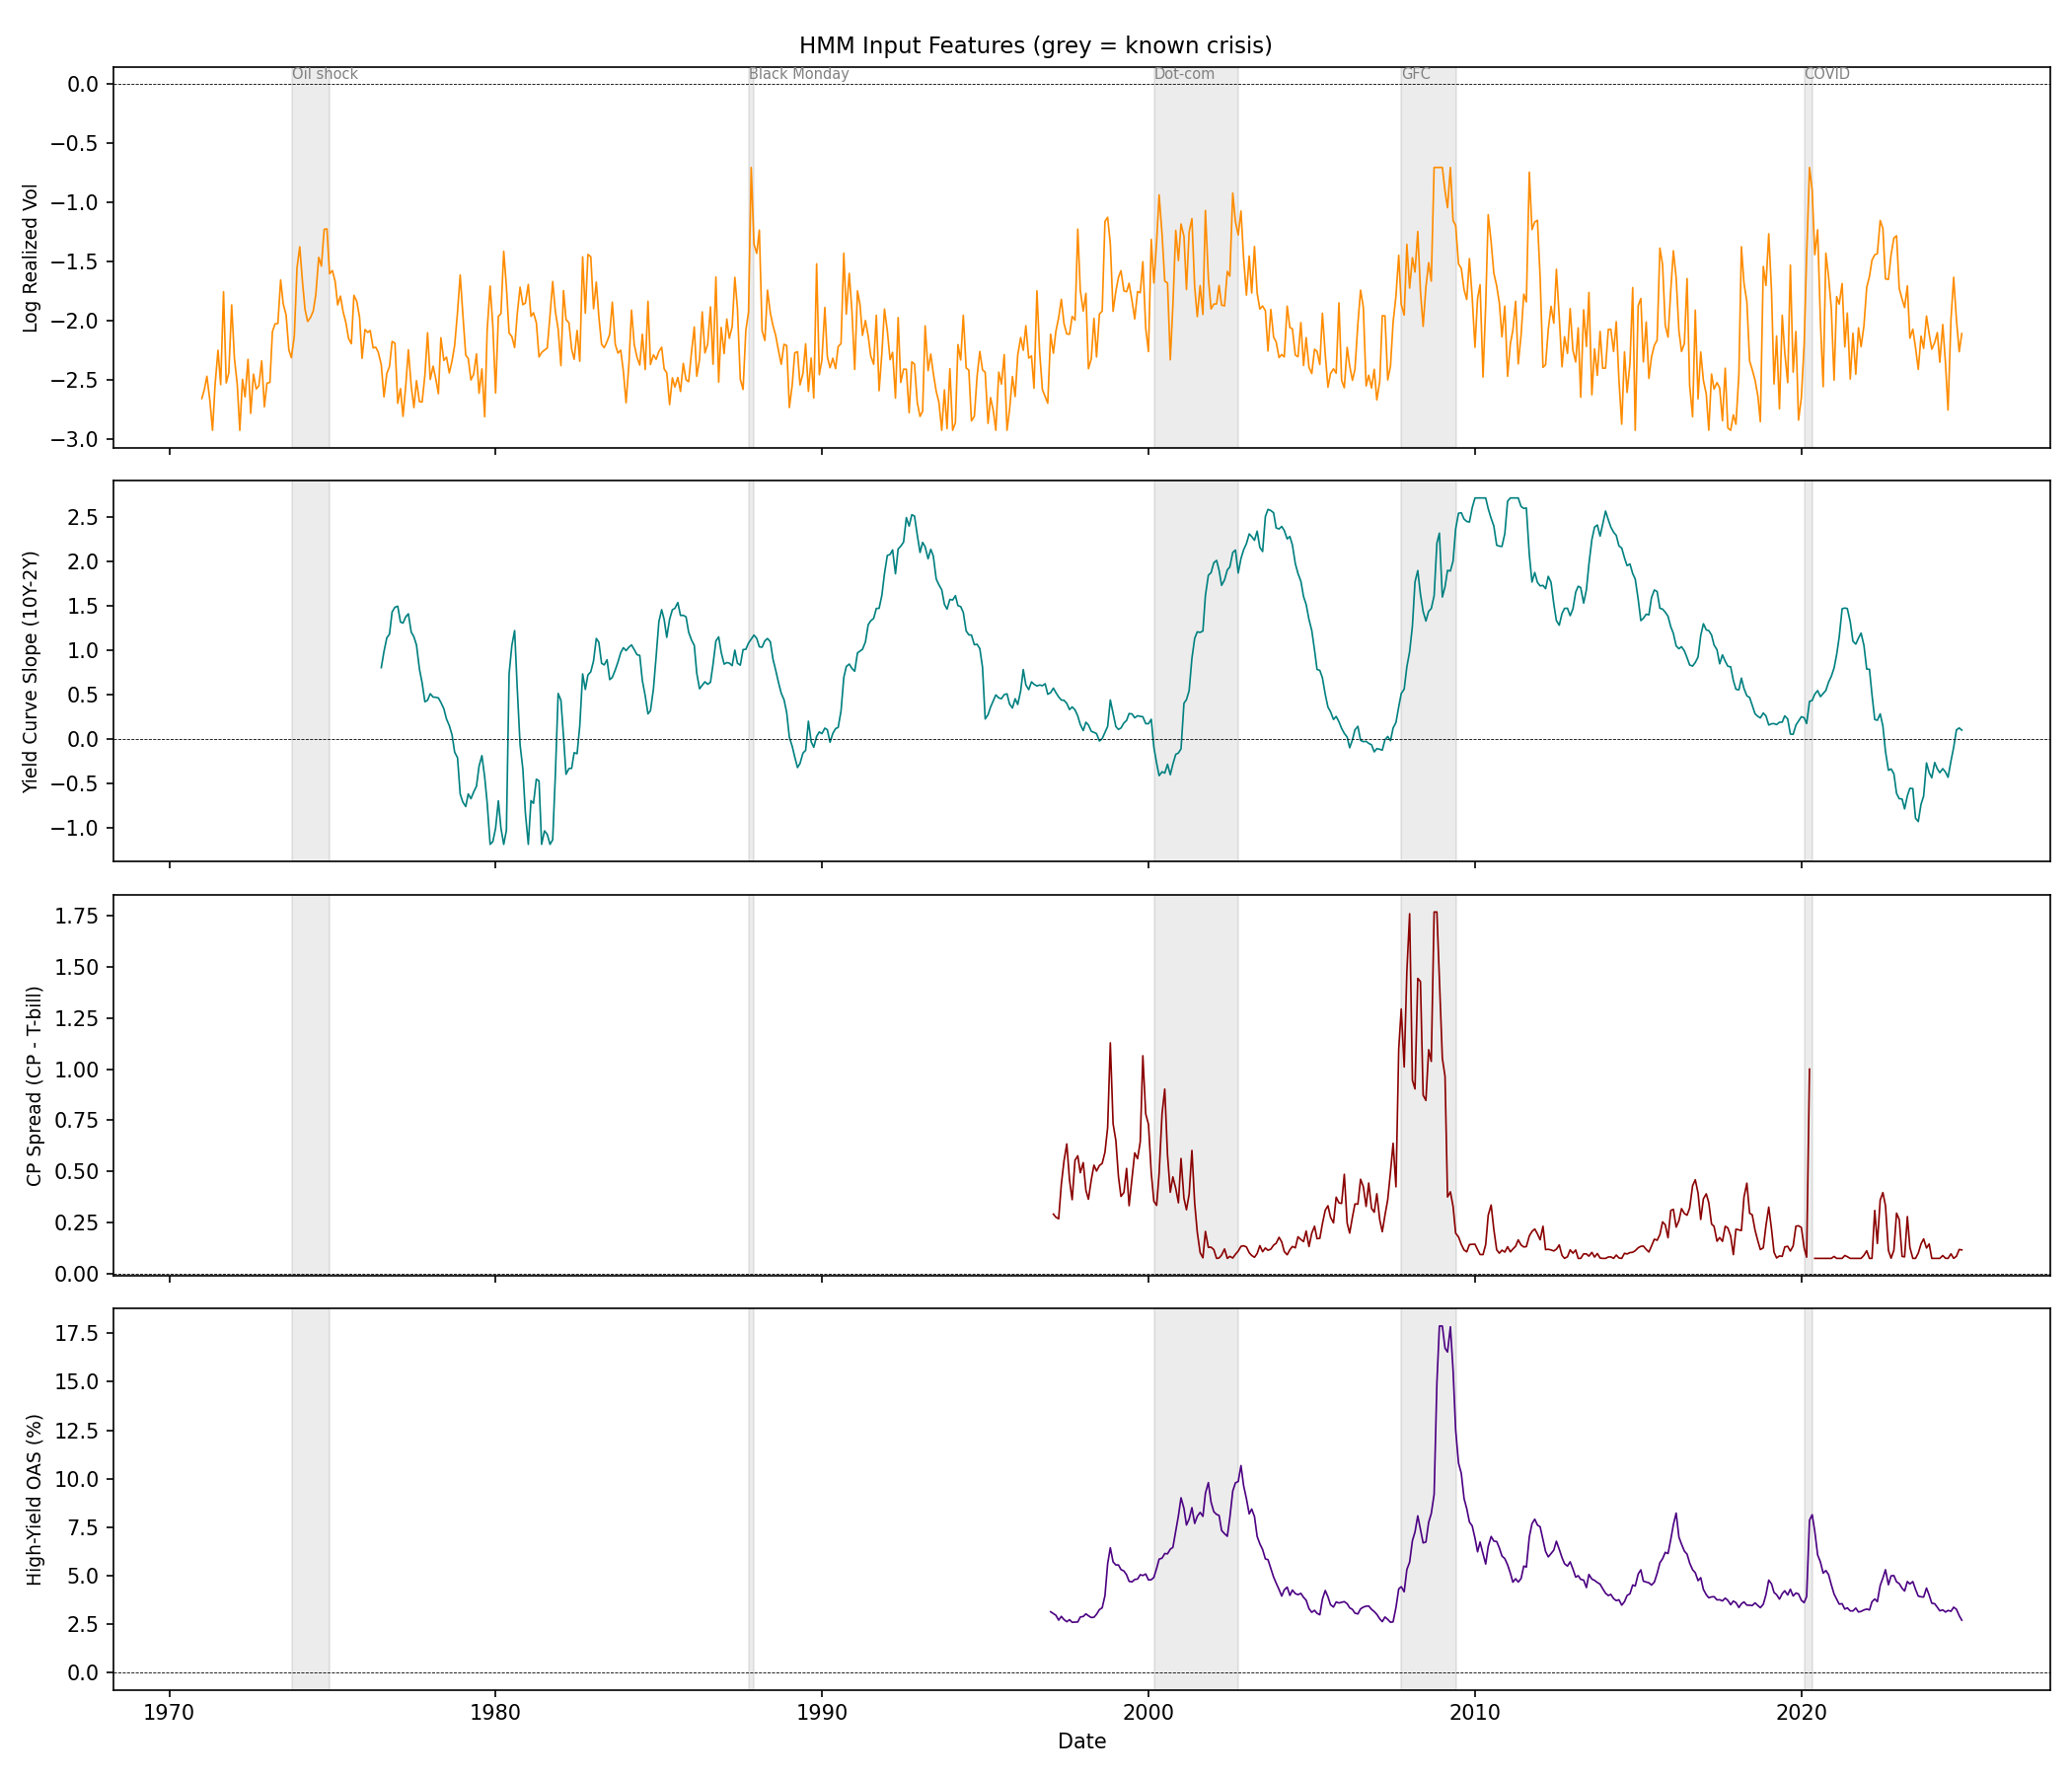
\includegraphics[width=\textwidth]{features_hmm.png}
    \caption{Time series of the four HMM input features (DD, DISP, REL\_N, CS), standardised using training-sample statistics. Shaded regions indicate NBER recession periods. All four features respond during the dot-com bust (2000--2002) and the global financial crisis (2007--2009), but with distinct dynamics reflecting their complementary stress dimensions.}
    \label{fig:features_hmm}
\end{figure}

\paragraph{Why these four features together}
The four selected indicators span complementary dimensions of market stress: DD captures the depth of equity market declines, DISP and REL\_N describe cross-sectional behaviour (stock disagreement and structural attrition), and CS captures corporate credit conditions. The feature selection procedure in Section~\ref{sec:feature_selection} confirms that this combination, drawn from a broader candidate pool of nine indicators including volatility and options market indicators, produces the most robust regime signal for the downstream momentum strategies.

\paragraph{Preprocessing}
All four features are winsorised at the 1st and 99th percentiles to limit the influence of extreme outliers.\footnote{Winsorisation replaces observations below the $p$-th percentile with the $p$-th percentile value, and observations above the $(1-p)$-th percentile with the $(1-p)$-th percentile value. Unlike trimming, which discards extreme observations entirely, winsorisation retains all data points while bounding their magnitude. This is particularly important for the HMM emission densities, which assume multivariate normality and can be distorted by heavy-tailed outliers.} The winsorisation bounds are computed on the training sample (1990--2010) and applied unchanged to the test sample, preventing information leakage. After winsorisation, each feature is standardised to zero mean and unit variance using training-sample statistics:
\begin{equation}
    z_{j,t} = \frac{x_{j,t} - \bar{x}_j^{\text{train}}}{\sigma_j^{\text{train}}}.
\end{equation}
Standardisation ensures that all features contribute equally to the HMM's Gaussian emission densities, so that the regime classification is not dominated by whichever feature has the largest raw scale.

\subsection{HMM Feature Selection}\label{sec:feature_selection}

The choice of HMM input features has a substantial impact on regime classification quality and, ultimately, on portfolio performance. This thesis selects features through a systematic three-pass pipeline that progressively filters candidates and increases computational rigor at each stage.

\paragraph{Candidate pool}
Nine monthly macrofinancial indicators, all available from 1990 onward, are considered as HMM inputs. These span three broad categories of market stress:
\begin{itemize}
    \item \emph{Equity market:} market drawdown (DD), realised volatility (VOL), cross-sectional return dispersion (DISP), relative market participation (REL\_N), advance-decline ratio (ADR), and cross-sectional return skewness (SKEW).
    \item \emph{Credit and macro:} BAA--AAA credit spread (CS), log VIX (LVIX), and the 10-year minus 2-year Treasury term spread (TERM).
\end{itemize}
All candidates are observable in real time at the end of each month. Two additional credit indicators (the commercial paper spread and the high-yield option-adjusted spread) are excluded because their data begins in the mid-1990s, providing insufficient training coverage for the 1990--2010 estimation window. All features are standardised to $z$-scores using training-period means and standard deviations, applied unchanged to the test period.

\paragraph{Pass~1: Quality screen}
Because market drawdown (DD) is the most economically direct measure of equity stress and consistently emerges as the dominant regime-identifying feature, it is required in every combination. The remaining eight candidates are combined with DD in groups of 1 to 3 additional features, yielding $1 + \binom{8}{1} + \binom{8}{2} + \binom{8}{3} = 93$ combinations spanning 1- to 4-feature HMMs. Each combination is estimated with a single Gibbs sampler seed (2{,}000 iterations, 500 burn-in). A combination passes the quality screen if it satisfies five criteria: (i)~minimum effective sample size (ESS) across all posterior mean parameters exceeds 50; (ii)~at least $\min(2, D)$ features exhibit statistically significant regime separation (95\% credible interval excluding zero); (iii)~the average filtered panic probability during the GFC (October 2007 to June 2009) exceeds 0.5 and during COVID (February to May 2020) exceeds 0.5; (iv)~the average panic probability during non-crisis reference periods (January 2003 to December 2006, and January 2013 to December 2019) remains below 0.4; and (v)~the Dot-com crash (March 2000 to October 2002) average exceeds 0.3. Panic state identification uses the same sign-correction method as the main HMM (Section~\ref{sec:gibbs}): the direction of each feature during known crises is determined empirically, and the state with the higher sign-corrected posterior mean is labelled as panic.

\paragraph{Pass~2: Portfolio ranking}
Surviving combinations are evaluated through the full cross-sectional pipeline. The filtered probability $\pi_t^{\text{filter}}$ is averaged across 5 HMM seeds to reduce MCMC noise. XGBoost predictions are averaged across 10 seeds to stabilise stock rankings. To maintain a fair comparison with the exposure-scaling approach of \citet{DanielMoskowitz2016}, portfolios use momentum and $\pi_t^{\text{filter}}$ only (no fundamental features) and are constructed as long-short with 10 basis points one-way costs applied to both legs. Combinations are ranked by out-of-sample Sharpe ratio. The top 10 advance to Pass~3.

\paragraph{Pass~3: Definitive validation}
The final pass increases seed counts to 10 HMM seeds and 20 XGBoost seeds. For each surviving combination, four tests are conducted:
\begin{enumerate}
    \item \emph{Ensemble Sharpe ratio} from the averaged predictions, representing the strategy's performance under heavy seed averaging.
    \item \emph{Sub-period consistency}: Sharpe ratios for 2011--2015, 2016--2020, and 2021--2025, verifying that performance is not driven by a single sub-period.
    \item \emph{Stability test}: 20 independent experiments, each using a random partition of 3 HMM seeds and 1 XGBoost seed drawn from a pool of 20, to assess sensitivity to the specific seed combination. Combinations are classified as stable ($\sigma < 0.10$), moderate ($0.10 \leq \sigma < 0.15$), or unstable ($\sigma \geq 0.15$).
    \item \emph{Leave-one-year-out}: each test-period year is dropped in turn to verify that no single year drives the result.
\end{enumerate}

\paragraph{Feature count comparison}
The pipeline evaluates combinations of 1 to 4 features to determine the optimal model complexity. Table~\ref{tab:feature_selection} reports the top combination at each feature count. Four features (DD+DISP+REL\_N+CS) achieves the highest stability mean (0.804) with the lowest standard deviation (0.082), indicating that the additional features reduce seed sensitivity without introducing overfitting. This combination is confirmed by a heavy variance test: 10 independent runs, each using 20 fresh HMM seeds (seeds 1--200) and 50 XGBoost seeds, produce a mean Sharpe of 0.804 with standard deviation 0.082.

\begin{table}[H]
\centering
\small
\begin{tabular}{c l r r r}
\toprule
$D$ & Combination & Sharpe & Mean & $\sigma$ \\
\midrule
4 & DD+DISP+REL\_N+CS & 0.91 & 0.84 & 0.11 \\
4 & DD+DISP+CS+TERM & 0.82 & 0.55 & 0.15 \\
4 & DD+DISP+REL\_N+SKEW & 0.80 & 0.69 & 0.08 \\
4 & DD+VOL+DISP+REL\_N & 0.80 & 0.77 & 0.09 \\
3 & DD+DISP+REL\_N & 0.77 & 0.77 & 0.10 \\
4 & DD+VOL+DISP+TERM & 0.71 & 0.67 & 0.16 \\
3 & DD+VOL+CS & 0.69 & 0.43 & 0.13 \\
1 & DD & 0.68 & 0.67 & 0.14 \\
4 & DD+DISP+REL\_N+TERM & 0.62 & 0.45 & 0.18 \\
3 & DD+ADR+TERM & 0.57 & 0.69 & 0.07 \\
\bottomrule
\end{tabular}
\caption{Top 10 feature combinations from the three-pass selection pipeline (long-short, 10 bps costs). $D$ = number of HMM features. Sharpe = ensemble Sharpe ratio (10 HMM seeds, 20 XGBoost seeds). Mean and $\sigma$ are the mean and standard deviation of the Sharpe ratio across 5 independent experiments with different seed partitions, measuring robustness to random initialisation. DD+DISP+REL\_N+CS ranks first on both ensemble Sharpe and stability mean.}
\label{tab:feature_selection}
\end{table}


\paragraph{Ablation analysis}
Single-feature and leave-one-out experiments isolate each feature's marginal contribution to the selected combination. DD alone achieves a Sharpe of 0.66, confirming its role as the dominant stress indicator. In the leave-one-out analysis, removing DD or REL\_N causes the largest performance drops ($-0.46$ and $-0.54$, respectively), while DISP and CS each contribute less than 0.01 marginally. Despite their small marginal contributions, DISP and CS improve the stability of the regime signal by providing independent information from different market segments (cross-sectional disagreement and corporate credit stress, respectively). The full ablation results are reported in Section~\ref{sec:ablation_results}.

\paragraph{Summary}
The selected feature set, DD+DISP+REL\_N+CS, captures market stress through three complementary dimensions: the depth of equity market declines (DD), cross-sectional stock disagreement (DISP) and structural market attrition (REL\_N), and corporate credit conditions (CS). All four features are available from January 1990, providing 241 training months that include both the dot-com crash and the global financial crisis. The final $\pi_t^{\text{filter}}$ used in all subsequent analyses is averaged across 200 HMM seeds and passes all three validation checks (regime separation, crisis alignment, and MCMC convergence).

\subsection{Cross-Sectional Features}\label{sec:cs_features}

The cross-sectional models use three groups of features to rank stocks each month: momentum signals, the filtered panic probability $\pi_t^{\text{filter}}$, and fundamental characteristics.

\paragraph{Momentum lookbacks}
Twelve trailing momentum signals are computed for each stock, corresponding to lookback horizons of 1 to 12 months:
\begin{equation}
    \text{mom}_{k,t}^s = \prod_{\ell=1}^{k}(1 + r_{t-\ell}^s) - 1, \qquad k = 1, \dots, 12,
\end{equation}
where $r_{t-\ell}^s$ is the adjusted return of stock $s$ in month $t - \ell$. Note that the current month's return is excluded from all lookbacks to avoid mechanical correlation with the forward return being predicted. Including all twelve horizons rather than a single lookback (e.g., the standard 12-month momentum of \citet{JegadeeshTitman1993}) allows the models to learn which horizons are most informative in each regime. As shown in Section~\ref{sec:ic_analysis}, intermediate-term lookbacks (8--11 months) dominate in calm markets, while 1-month momentum becomes important during panic due to short-term reversal dynamics.

\paragraph{Regime signal}
The filtered panic probability $\pi_t^{\text{filter}}$ from the HMM enters as a single feature. Because it varies only at the monthly market level (every stock in the same month receives the same value), it functions as a conditioning variable rather than a stock-level predictor. Its role in the cross-sectional models is discussed in Section~\ref{sec:ic_analysis}.

\paragraph{Fundamental characteristics}
Seven firm-level characteristics are computed from Compustat quarterly data. These variables are drawn from the established asset pricing literature: book-to-market and size are the original \citet{FamaFrench2015} factors, gross profitability follows \citet{NovyMarx2013}, and the remaining variables (leverage, asset growth, return on equity, earnings growth) capture investment and quality dimensions that have been shown to predict cross-sectional returns. Their role in the models is not to generate additional returns but to act as a quality screen that compresses portfolio volatility (see Section~\ref{sec:performance_results}).

\begin{itemize}
    \item \textbf{Book-to-market (bm):} Book equity divided by market equity, $\text{ceqq} / ME$. Captures the value premium.
    \item \textbf{Return on equity (roe):} Income before extraordinary items divided by book equity, $\text{ibq} / \text{ceqq}$. Measures profitability.
    \item \textbf{Gross profitability:} Revenue minus cost of goods sold, scaled by total assets, $(\text{revtq} - \text{cogsq}) / \text{atq}$. Follows the profitability factor of \citet{NovyMarx2013}.
    \item \textbf{Asset growth:} Year-over-year growth in total assets, $\text{atq}_t / \text{atq}_{t-4} - 1$. Firms with high asset growth tend to have lower future returns.
    \item \textbf{Leverage:} Total debt divided by total assets, $(\text{dlttq} + \text{dlcq}) / \text{atq}$. Highly leveraged firms are more vulnerable to financial distress.
    \item \textbf{Earnings growth:} Year-over-year growth in earnings, computed as $\text{sign}(g) \cdot \log(1 + |g|)$ where $g = \text{ibq}_t / \text{ibq}_{t-4} - 1$. The signed-log transformation handles the fat-tailed distribution of earnings changes.
    \item \textbf{Log market equity:} The natural logarithm of market capitalisation (price times shares outstanding), lagged one month. Controls for the size effect.
\end{itemize}

Market equity is computed as the absolute value of the end-of-month stock price multiplied by shares outstanding from CRSP. The absolute value handles cases where CRSP reports the bid-ask midpoint as a negative price.

All fundamental variables are lagged by four months relative to the fiscal quarter end to ensure that accounting data would have been publicly available at the time of portfolio formation, consistent with the standard approach in the empirical asset pricing literature. This lag accounts for the SEC filing deadline and prevents look-ahead bias. Each month, the most recent available quarter's fundamentals are assigned to each stock using a backward merge, so that no future accounting information is used. Fundamentals are winsorised at the 1st and 99th percentiles (5th and 95th for asset growth, which has a fatter right tail), with bounds computed on the training sample only.

\paragraph{Missing data handling}
Not all stocks have complete fundamental coverage in every month. Missing rates range from approximately 7\% (return on equity, leverage) to 17\% (gross profitability). For the logistic regression model, which cannot handle missing values, fundamentals are imputed at the training-sample median prior to standardisation. For XGBoost, which natively handles missing values by learning optimal split directions for absent features, no imputation is applied. In both cases, stocks are only excluded if core features (momentum lookbacks or the regime signal) are missing.

\subsection{Train--Test Split and Information Leakage Prevention}\label{sec:split}

The sample is divided at December 2010. The HMM start date of January 1990 is determined by the availability of sufficient stock-level data for computing cross-sectional return dispersion, and the split point is chosen so that the training period contains at least two full market cycles, including the dot-com crash (2000--2002) and the global financial crisis (2007--2009), giving the HMM sufficient exposure to both calm and panic regimes. The training period is used for all model estimation: HMM Gibbs sampling, logistic regression fitting, and XGBoost training. The test period (January 2011 to November 2025, 167 months) is reserved exclusively for out-of-sample evaluation; no model parameters are re-estimated or updated during this period.

Several safeguards prevent information leakage from the test period into model training:
\begin{itemize}
    \item Winsorisation bounds and standardisation statistics (means, standard deviations) are computed on the training sample and applied unchanged to the test sample.
    \item The HMM posterior mean parameters (regime means $\boldsymbol{\mu}_k$, covariances $\boldsymbol{\Sigma}_k$, and transition matrix $\mathbf{P}$) are estimated on the training period and frozen. During the test period, only the forward-filtering recursion is run using the fixed parameters, producing the causal signal $\pi_t^{\text{filter}}$ without any parameter updating.
    \item The cross-sectional models are trained once on the training sample and applied without retraining to the test sample.
    \item NYSE breakpoints for portfolio decile assignment are computed each month using only NYSE-listed stocks in that month, which is observable in real time.
\end{itemize}

A single fixed split is standard in the literature that this thesis builds on \citep[e.g.,][]{GHM2023} and is appropriate given the computational cost of re-estimating the Bayesian HMM via Gibbs sampling. Alternative train/test splits (Appendix~\ref{app:alt_splits}) confirm that both M1 and M2 produce positive Sharpe ratios across all splits tested, though the baseline split yields the strongest M1 performance. The 14-year out-of-sample test period and the statistical significance tests reported in Section~\ref{sec:performance_results} further mitigate concerns about split dependence.
 from main.tex
%% ═══════════════════════════════════════════════════════════════════════════

\section{Data}\label{sec:data}

The data sources, sample construction, and feature definitions used throughout the thesis are described below. All data are at the monthly frequency. The stock-level sample spans January 1990 to November 2025, while the HMM regime model uses data from January 1990 onward (determined by the availability of stock-level data for computing cross-sectional return dispersion and relative market participation). The sample is split into a training period (pre-2011) used to estimate the HMM and cross-sectional models, and an out-of-sample test period (2011--2025) used exclusively for performance evaluation. Table~\ref{tab:sample_summary} provides an overview of the sample.

\begin{table}[H]
\centering
\begin{tabular}{l r r r}
\toprule
 & Train (1990--2010) & Test (2011--2025) & Full \\
\midrule
Unique stocks & 15{,}232 & 7{,}473 & 18{,}700 \\
Stock-month observations & 1{,}442{,}168 & 640{,}317 & 2{,}082{,}485 \\
Avg.\ stocks per month & 5{,}723 & 3{,}811 & 4{,}958 \\
Market-level months & 252 & 167 & 419 \\
\bottomrule
\end{tabular}
\caption{Sample summary.}
\label{tab:sample_summary}

\medskip
\small
\textbf{Notes:} The sample includes all ordinary common shares (CRSP share codes 10 and 11) listed on the NYSE, AMEX, or NASDAQ with a price above \$1. The decline in the average number of stocks in the test period reflects ongoing market consolidation and tighter listing standards.
\end{table}

\subsection{Data Sources}\label{sec:data_sources}

Three primary data sources are used:

\begin{itemize}
    \item \textbf{CRSP} (Center for Research in Security Prices, accessed via WRDS): Monthly stock-level returns, prices, shares outstanding, exchange codes, and share codes from the Monthly Stock File (\texttt{crsp.msf}). Daily market returns from the Daily Stock Index file (\texttt{crsp.dsi}) are used to compute the market drawdown feature. Delisting returns from \texttt{crsp.msedelist} are incorporated to avoid survivorship bias.
    \item \textbf{Compustat} (accessed via WRDS): Quarterly fundamental accounting data from \texttt{comp.fundq}, linked to CRSP via the CCM bridge table (\texttt{crsp.ccmxpf\_lnkhist}) using primary link types (LU, LC) with primary link indicators (P, C). Only observations where the fiscal quarter date falls within the active link window are retained. Variables include book equity (\texttt{ceqq}), total assets (\texttt{atq}), income before extraordinary items (\texttt{ibq}), revenue (\texttt{revtq}), cost of goods sold (\texttt{cogsq}), and debt (\texttt{dlttq}, \texttt{dlcq}).
    \item \textbf{FRED} (Federal Reserve Economic Data): Moody's BAA and AAA corporate bond yields, used to compute the credit spread (CS) that enters the final HMM specification (see Section~\ref{sec:feature_selection}). The CBOE Volatility Index (VIX) was also evaluated as a candidate but was not selected. The HMM sample begins in 1990, determined by the availability of stock-level data for computing cross-sectional return dispersion and relative market participation.
\end{itemize}

\subsection{Stock Universe and Filtering}\label{sec:stock_universe}

The stock-level sample includes all ordinary common shares (CRSP share codes 10 and 11) listed on the NYSE, AMEX, or NASDAQ (exchange codes 1, 2, and 3). This excludes American Depositary Receipts (ADRs), Real Estate Investment Trusts (REITs), closed-end funds, and other non-standard securities. A minimum price filter of \$1 is applied to remove penny stocks, whose extreme percentage returns and low liquidity would distort momentum signals.\footnote{This filter is standard in the momentum literature; see, e.g., \citet{JegadeeshTitman2001}. Stocks priced below \$1 can exhibit percentage returns of hundreds of percent from small absolute price changes, contaminating momentum signals.}

\paragraph{Delisting adjustment}
Following \citet{Shumway2001}, delisting returns are incorporated to prevent survivorship bias. When a stock is delisted, its actual delisting return is used if available; for performance-related delistings (CRSP codes 500--584) with missing returns, $-30\%$ is imputed.

\subsection{HMM Regime Features}\label{sec:hmm_features}

The Hidden Markov Model takes as input four macrofinancial stress indicators, selected through the systematic procedure described in Section~\ref{sec:feature_selection}. All four indicators are \textbf{observable in real time} at the end of each month.\footnote{``Real time'' means that each feature can be computed from data available on the last trading day of the month, with no reporting lag or subsequent revision. This is in contrast to macroeconomic indicators such as GDP, which are released with a delay and revised multiple times.} This real-time availability is essential: because the filtered regime probability $\pi_t^{\text{filter}}$ is used as a trading signal, any feature with a reporting lag would introduce look-ahead bias. Indicators such as GDP growth, which is published with a delay of approximately one month and subject to subsequent revisions, are therefore excluded despite their economic relevance.

The four features are:

\begin{enumerate}
    \item \textbf{DD (Drawdown):} The percentage decline of the cumulative market price index from its rolling 12-month peak:
    \begin{equation}
        DD_t = \frac{P_t - \max(P_{t-11}, \dots, P_t)}{\max(P_{t-11}, \dots, P_t)},
    \end{equation}
    where $P_t = 100 \times \prod_{\tau=1}^{t}(1 + r_\tau^{\text{mkt}})$ is the cumulative value-weighted market return index. DD is always non-positive and captures the magnitude of an ongoing downturn. \citet{DanielMoskowitz2016} show that the conditional volatility of momentum strategies is strongly related to past market declines, as drawdowns trigger forced selling and margin calls that reverse momentum profits. DD directly measures this mechanism and, as shown in Section~\ref{sec:ablation_results}, is the single most informative HMM input feature for downstream portfolio performance.

    \item \textbf{DISP (Return Dispersion):} The log cross-sectional standard deviation of individual stock returns within each month:
    \begin{equation}
        DISP_t = \log\!\left(\text{std}_s(r_{s,t})\right),
    \end{equation}
    where $\text{std}_s$ denotes the standard deviation computed across all stocks $s$ in the universe in month~$t$. Return dispersion captures cross-sectional \emph{disagreement} among individual stocks. During stress, consensus breaks down and dispersion spikes, signalling changes in the correlation structure that affect momentum profits.

    \item \textbf{REL\_N (Relative Market Participation):} The log ratio of the number of actively traded stocks in month~$t$ to its trailing 12-month moving average:
    \begin{equation}
        REL\_N_t = \log\!\left(\frac{N_t}{\frac{1}{12}\sum_{\ell=1}^{12} N_{t-\ell}}\right),
    \end{equation}
    where $N_t$ is the number of stocks with valid return observations in month~$t$. REL\_N is close to zero in normal times but turns negative during crises when stocks delist, halt trading, or are acquired at elevated rates. For example, during the 2008 financial crisis, a wave of delistings and trading halts caused $N_t$ to drop sharply relative to its trailing average. This captures structural market damage that the other three features do not measure.

    \item \textbf{CS (Credit Spread):} The difference between Moody's BAA and AAA corporate bond yields:
    \begin{equation}
        CS_t = Y_t^{\text{BAA}} - Y_t^{\text{AAA}}.
    \end{equation}
    The credit spread widens when investors demand higher compensation for default risk, making it a leading indicator of financial stress that is distinct from the equity-based features above. Unlike DD, DISP, and REL\_N, which are derived entirely from equity market data, CS provides an independent signal from the corporate bond market. This cross-market information helps the HMM distinguish genuine stress episodes from equity-specific turbulence.
\end{enumerate}

\begin{figure}[H]
    \centering
    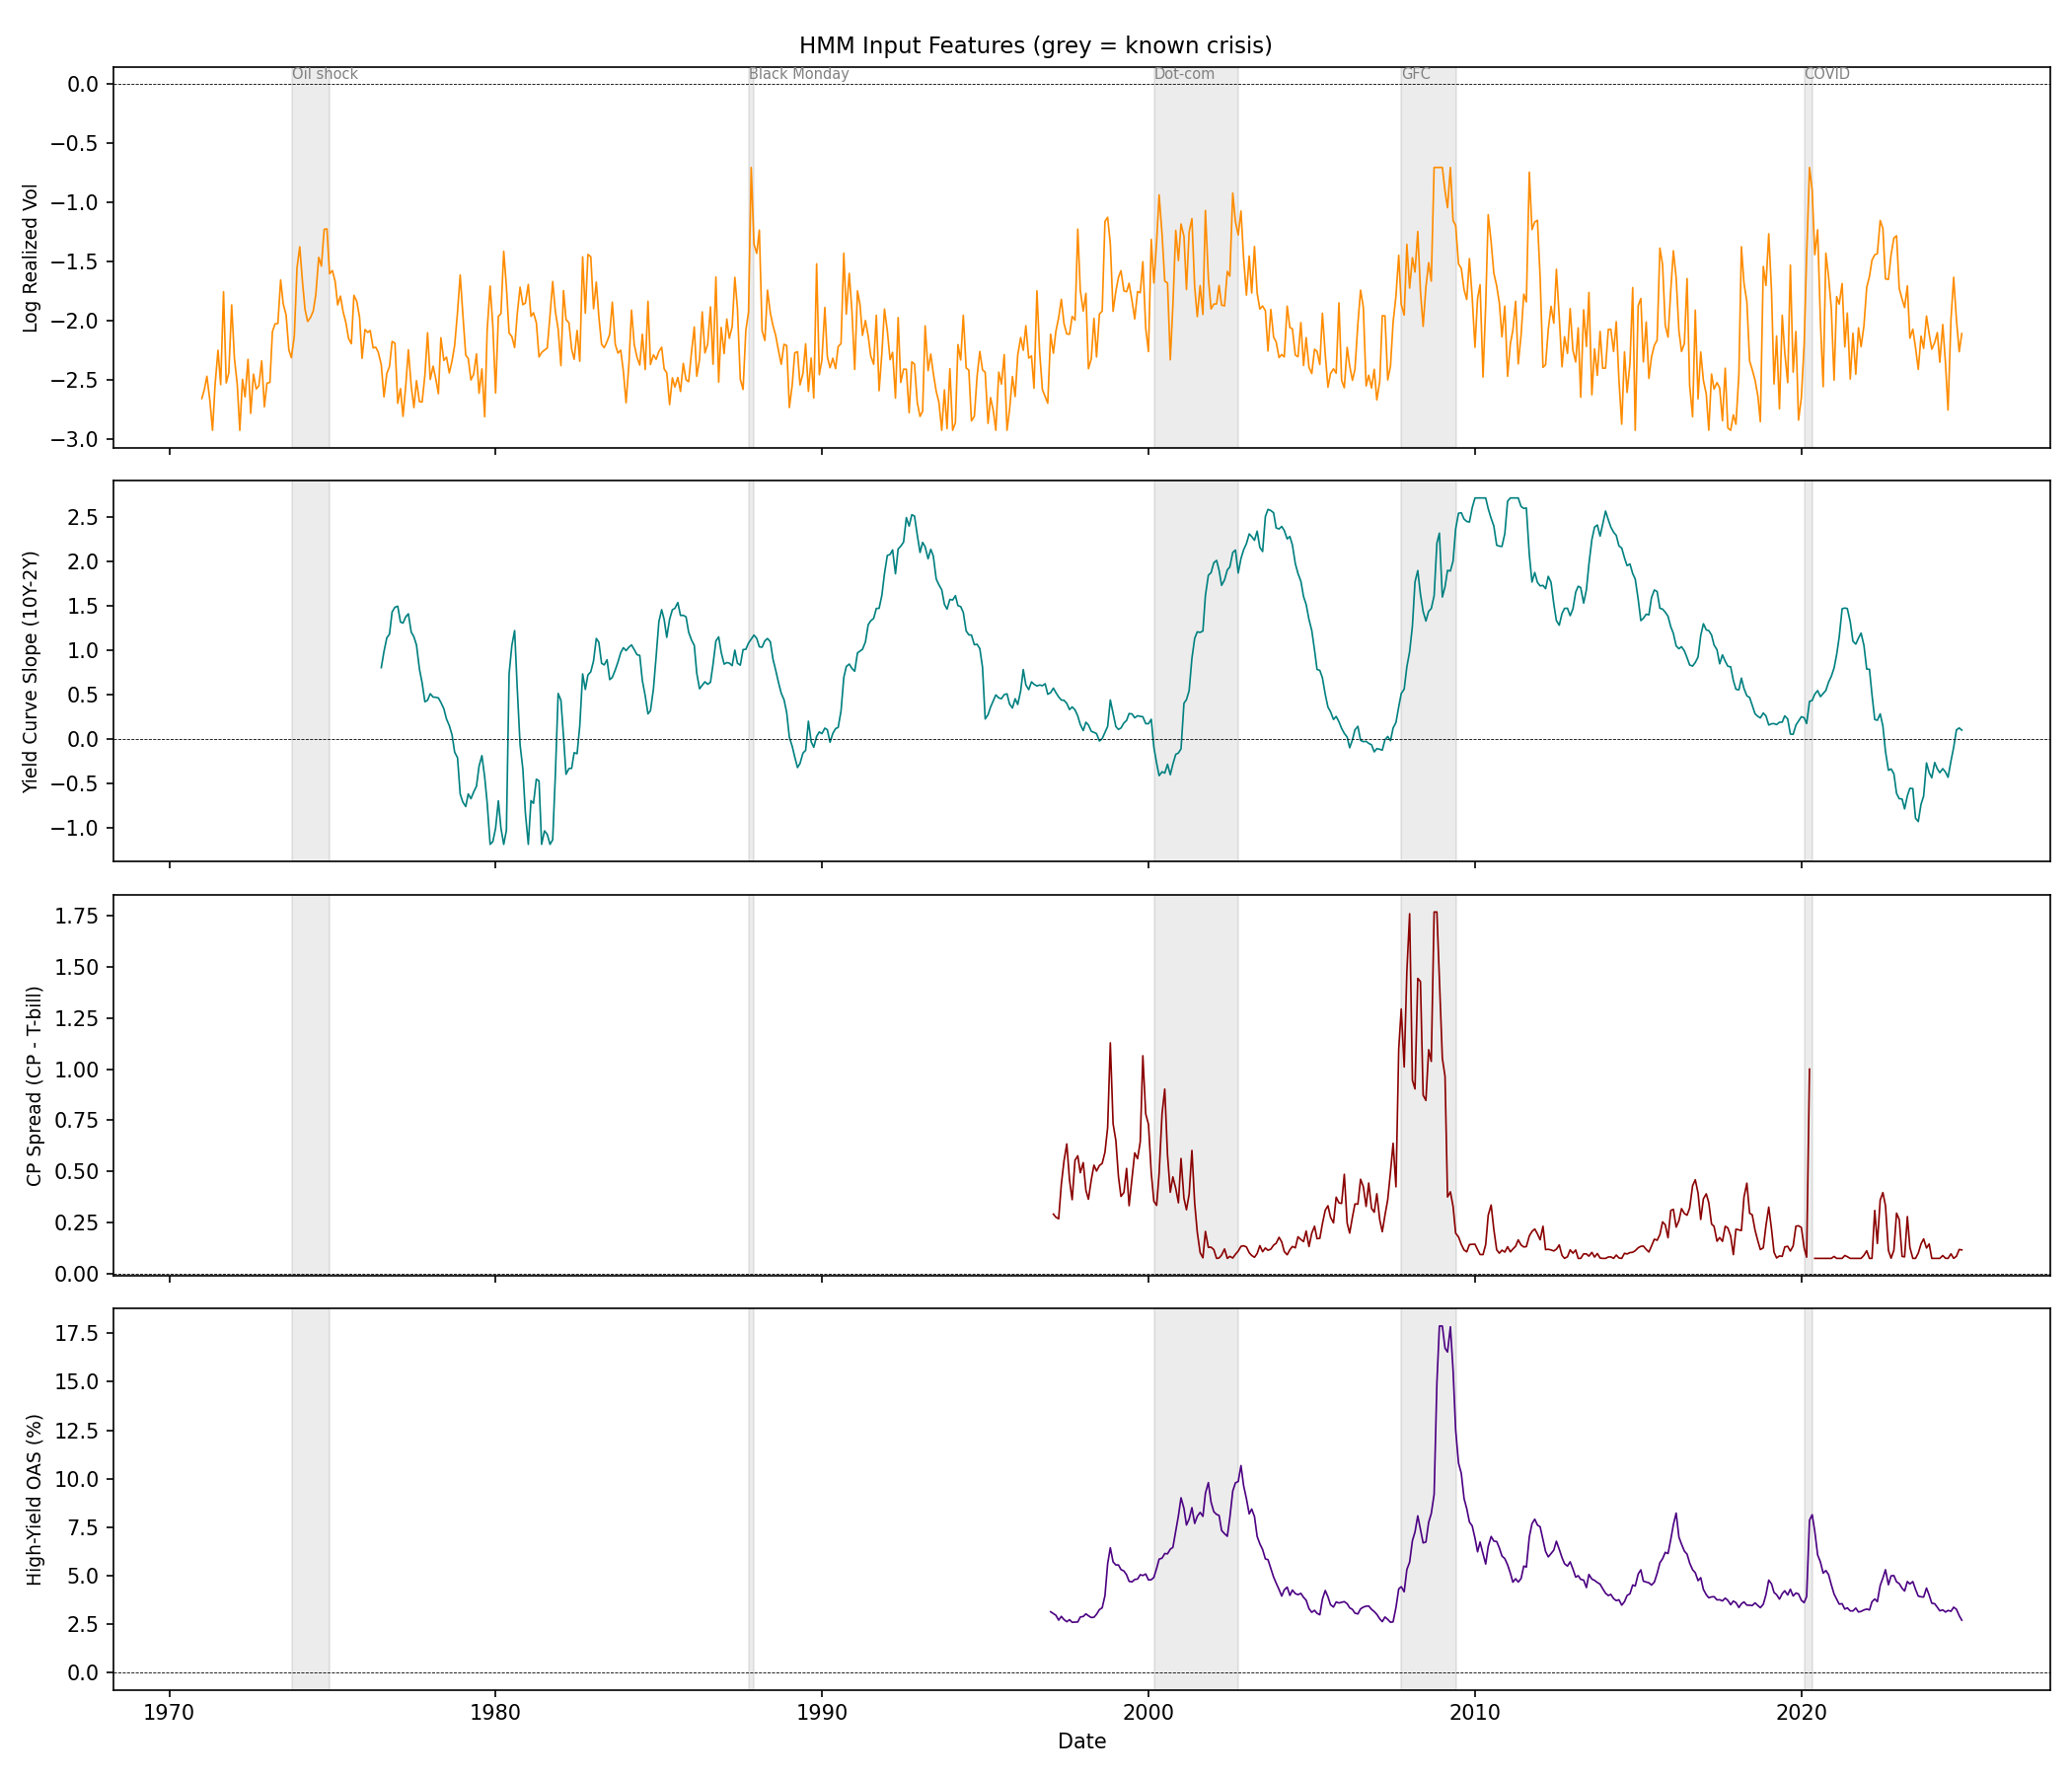
\includegraphics[width=\textwidth]{features_hmm.png}
    \caption{Time series of the four HMM input features (DD, DISP, REL\_N, CS), standardised using training-sample statistics. Shaded regions indicate NBER recession periods. All four features respond during the dot-com bust (2000--2002) and the global financial crisis (2007--2009), but with distinct dynamics reflecting their complementary stress dimensions.}
    \label{fig:features_hmm}
\end{figure}

\paragraph{Why these four features together}
The four selected indicators span complementary dimensions of market stress: DD captures the depth of equity market declines, DISP and REL\_N describe cross-sectional behaviour (stock disagreement and structural attrition), and CS captures corporate credit conditions. The feature selection procedure in Section~\ref{sec:feature_selection} confirms that this combination, drawn from a broader candidate pool of nine indicators including volatility and options market indicators, produces the most robust regime signal for the downstream momentum strategies.

\paragraph{Preprocessing}
All four features are winsorised at the 1st and 99th percentiles to limit the influence of extreme outliers.\footnote{Winsorisation replaces observations below the $p$-th percentile with the $p$-th percentile value, and observations above the $(1-p)$-th percentile with the $(1-p)$-th percentile value. Unlike trimming, which discards extreme observations entirely, winsorisation retains all data points while bounding their magnitude. This is particularly important for the HMM emission densities, which assume multivariate normality and can be distorted by heavy-tailed outliers.} The winsorisation bounds are computed on the training sample (1990--2010) and applied unchanged to the test sample, preventing information leakage. After winsorisation, each feature is standardised to zero mean and unit variance using training-sample statistics:
\begin{equation}
    z_{j,t} = \frac{x_{j,t} - \bar{x}_j^{\text{train}}}{\sigma_j^{\text{train}}}.
\end{equation}
Standardisation ensures that all features contribute equally to the HMM's Gaussian emission densities, so that the regime classification is not dominated by whichever feature has the largest raw scale.

\subsection{HMM Feature Selection}\label{sec:feature_selection}

The choice of HMM input features has a substantial impact on regime classification quality and, ultimately, on portfolio performance. This thesis selects features through a systematic three-pass pipeline that progressively filters candidates and increases computational rigor at each stage.

\paragraph{Candidate pool}
Nine monthly macrofinancial indicators, all available from 1990 onward, are considered as HMM inputs. These span three broad categories of market stress:
\begin{itemize}
    \item \emph{Equity market:} market drawdown (DD), realised volatility (VOL), cross-sectional return dispersion (DISP), relative market participation (REL\_N), advance-decline ratio (ADR), and cross-sectional return skewness (SKEW).
    \item \emph{Credit and macro:} BAA--AAA credit spread (CS), log VIX (LVIX), and the 10-year minus 2-year Treasury term spread (TERM).
\end{itemize}
All candidates are observable in real time at the end of each month. Two additional credit indicators (the commercial paper spread and the high-yield option-adjusted spread) are excluded because their data begins in the mid-1990s, providing insufficient training coverage for the 1990--2010 estimation window. All features are standardised to $z$-scores using training-period means and standard deviations, applied unchanged to the test period.

\paragraph{Pass~1: Quality screen}
Because market drawdown (DD) is the most economically direct measure of equity stress and consistently emerges as the dominant regime-identifying feature, it is required in every combination. The remaining eight candidates are combined with DD in groups of 1 to 3 additional features, yielding $1 + \binom{8}{1} + \binom{8}{2} + \binom{8}{3} = 93$ combinations spanning 1- to 4-feature HMMs. Each combination is estimated with a single Gibbs sampler seed (2{,}000 iterations, 500 burn-in). A combination passes the quality screen if it satisfies five criteria: (i)~minimum effective sample size (ESS) across all posterior mean parameters exceeds 50; (ii)~at least $\min(2, D)$ features exhibit statistically significant regime separation (95\% credible interval excluding zero); (iii)~the average filtered panic probability during the GFC (October 2007 to June 2009) exceeds 0.5 and during COVID (February to May 2020) exceeds 0.5; (iv)~the average panic probability during non-crisis reference periods (January 2003 to December 2006, and January 2013 to December 2019) remains below 0.4; and (v)~the Dot-com crash (March 2000 to October 2002) average exceeds 0.3. Panic state identification uses the same sign-correction method as the main HMM (Section~\ref{sec:gibbs}): the direction of each feature during known crises is determined empirically, and the state with the higher sign-corrected posterior mean is labelled as panic.

\paragraph{Pass~2: Portfolio ranking}
Surviving combinations are evaluated through the full cross-sectional pipeline. The filtered probability $\pi_t^{\text{filter}}$ is averaged across 5 HMM seeds to reduce MCMC noise. XGBoost predictions are averaged across 10 seeds to stabilise stock rankings. To maintain a fair comparison with the exposure-scaling approach of \citet{DanielMoskowitz2016}, portfolios use momentum and $\pi_t^{\text{filter}}$ only (no fundamental features) and are constructed as long-short with 10 basis points one-way costs applied to both legs. Combinations are ranked by out-of-sample Sharpe ratio. The top 10 advance to Pass~3.

\paragraph{Pass~3: Definitive validation}
The final pass increases seed counts to 10 HMM seeds and 20 XGBoost seeds. For each surviving combination, four tests are conducted:
\begin{enumerate}
    \item \emph{Ensemble Sharpe ratio} from the averaged predictions, representing the strategy's performance under heavy seed averaging.
    \item \emph{Sub-period consistency}: Sharpe ratios for 2011--2015, 2016--2020, and 2021--2025, verifying that performance is not driven by a single sub-period.
    \item \emph{Stability test}: 20 independent experiments, each using a random partition of 3 HMM seeds and 1 XGBoost seed drawn from a pool of 20, to assess sensitivity to the specific seed combination. Combinations are classified as stable ($\sigma < 0.10$), moderate ($0.10 \leq \sigma < 0.15$), or unstable ($\sigma \geq 0.15$).
    \item \emph{Leave-one-year-out}: each test-period year is dropped in turn to verify that no single year drives the result.
\end{enumerate}

\paragraph{Feature count comparison}
The pipeline evaluates combinations of 1 to 4 features to determine the optimal model complexity. Table~\ref{tab:feature_selection} reports the top combination at each feature count. Four features (DD+DISP+REL\_N+CS) achieves the highest stability mean (0.804) with the lowest standard deviation (0.082), indicating that the additional features reduce seed sensitivity without introducing overfitting. This combination is confirmed by a heavy variance test: 10 independent runs, each using 20 fresh HMM seeds (seeds 1--200) and 50 XGBoost seeds, produce a mean Sharpe of 0.804 with standard deviation 0.082.

\begin{table}[H]
\centering
\small
\begin{tabular}{c l r r r}
\toprule
$D$ & Combination & Sharpe & Mean & $\sigma$ \\
\midrule
4 & DD+DISP+REL\_N+CS & 0.91 & 0.84 & 0.11 \\
4 & DD+DISP+CS+TERM & 0.82 & 0.55 & 0.15 \\
4 & DD+DISP+REL\_N+SKEW & 0.80 & 0.69 & 0.08 \\
4 & DD+VOL+DISP+REL\_N & 0.80 & 0.77 & 0.09 \\
3 & DD+DISP+REL\_N & 0.77 & 0.77 & 0.10 \\
4 & DD+VOL+DISP+TERM & 0.71 & 0.67 & 0.16 \\
3 & DD+VOL+CS & 0.69 & 0.43 & 0.13 \\
1 & DD & 0.68 & 0.67 & 0.14 \\
4 & DD+DISP+REL\_N+TERM & 0.62 & 0.45 & 0.18 \\
3 & DD+ADR+TERM & 0.57 & 0.69 & 0.07 \\
\bottomrule
\end{tabular}
\caption{Top 10 feature combinations from the three-pass selection pipeline (long-short, 10 bps costs). $D$ = number of HMM features. Sharpe = ensemble Sharpe ratio (10 HMM seeds, 20 XGBoost seeds). Mean and $\sigma$ are the mean and standard deviation of the Sharpe ratio across 5 independent experiments with different seed partitions, measuring robustness to random initialisation. DD+DISP+REL\_N+CS ranks first on both ensemble Sharpe and stability mean.}
\label{tab:feature_selection}
\end{table}


\paragraph{Ablation analysis}
Single-feature and leave-one-out experiments isolate each feature's marginal contribution to the selected combination. DD alone achieves a Sharpe of 0.66, confirming its role as the dominant stress indicator. In the leave-one-out analysis, removing DD or REL\_N causes the largest performance drops ($-0.46$ and $-0.54$, respectively), while DISP and CS each contribute less than 0.01 marginally. Despite their small marginal contributions, DISP and CS improve the stability of the regime signal by providing independent information from different market segments (cross-sectional disagreement and corporate credit stress, respectively). The full ablation results are reported in Section~\ref{sec:ablation_results}.

\paragraph{Summary}
The selected feature set, DD+DISP+REL\_N+CS, captures market stress through three complementary dimensions: the depth of equity market declines (DD), cross-sectional stock disagreement (DISP) and structural market attrition (REL\_N), and corporate credit conditions (CS). All four features are available from January 1990, providing 241 training months that include both the dot-com crash and the global financial crisis. The final $\pi_t^{\text{filter}}$ used in all subsequent analyses is averaged across 200 HMM seeds and passes all three validation checks (regime separation, crisis alignment, and MCMC convergence).

\subsection{Cross-Sectional Features}\label{sec:cs_features}

The cross-sectional models use three groups of features to rank stocks each month: momentum signals, the filtered panic probability $\pi_t^{\text{filter}}$, and fundamental characteristics.

\paragraph{Momentum lookbacks}
Twelve trailing momentum signals are computed for each stock, corresponding to lookback horizons of 1 to 12 months:
\begin{equation}
    \text{mom}_{k,t}^s = \prod_{\ell=1}^{k}(1 + r_{t-\ell}^s) - 1, \qquad k = 1, \dots, 12,
\end{equation}
where $r_{t-\ell}^s$ is the adjusted return of stock $s$ in month $t - \ell$. Note that the current month's return is excluded from all lookbacks to avoid mechanical correlation with the forward return being predicted. Including all twelve horizons rather than a single lookback (e.g., the standard 12-month momentum of \citet{JegadeeshTitman1993}) allows the models to learn which horizons are most informative in each regime. As shown in Section~\ref{sec:ic_analysis}, intermediate-term lookbacks (8--11 months) dominate in calm markets, while 1-month momentum becomes important during panic due to short-term reversal dynamics.

\paragraph{Regime signal}
The filtered panic probability $\pi_t^{\text{filter}}$ from the HMM enters as a single feature. Because it varies only at the monthly market level (every stock in the same month receives the same value), it functions as a conditioning variable rather than a stock-level predictor. Its role in the cross-sectional models is discussed in Section~\ref{sec:ic_analysis}.

\paragraph{Fundamental characteristics}
Seven firm-level characteristics are computed from Compustat quarterly data. These variables are drawn from the established asset pricing literature: book-to-market and size are the original \citet{FamaFrench2015} factors, gross profitability follows \citet{NovyMarx2013}, and the remaining variables (leverage, asset growth, return on equity, earnings growth) capture investment and quality dimensions that have been shown to predict cross-sectional returns. Their role in the models is not to generate additional returns but to act as a quality screen that compresses portfolio volatility (see Section~\ref{sec:performance_results}).

\begin{itemize}
    \item \textbf{Book-to-market (bm):} Book equity divided by market equity, $\text{ceqq} / ME$. Captures the value premium.
    \item \textbf{Return on equity (roe):} Income before extraordinary items divided by book equity, $\text{ibq} / \text{ceqq}$. Measures profitability.
    \item \textbf{Gross profitability:} Revenue minus cost of goods sold, scaled by total assets, $(\text{revtq} - \text{cogsq}) / \text{atq}$. Follows the profitability factor of \citet{NovyMarx2013}.
    \item \textbf{Asset growth:} Year-over-year growth in total assets, $\text{atq}_t / \text{atq}_{t-4} - 1$. Firms with high asset growth tend to have lower future returns.
    \item \textbf{Leverage:} Total debt divided by total assets, $(\text{dlttq} + \text{dlcq}) / \text{atq}$. Highly leveraged firms are more vulnerable to financial distress.
    \item \textbf{Earnings growth:} Year-over-year growth in earnings, computed as $\text{sign}(g) \cdot \log(1 + |g|)$ where $g = \text{ibq}_t / \text{ibq}_{t-4} - 1$. The signed-log transformation handles the fat-tailed distribution of earnings changes.
    \item \textbf{Log market equity:} The natural logarithm of market capitalisation (price times shares outstanding), lagged one month. Controls for the size effect.
\end{itemize}

Market equity is computed as the absolute value of the end-of-month stock price multiplied by shares outstanding from CRSP. The absolute value handles cases where CRSP reports the bid-ask midpoint as a negative price.

All fundamental variables are lagged by four months relative to the fiscal quarter end to ensure that accounting data would have been publicly available at the time of portfolio formation, consistent with the standard approach in the empirical asset pricing literature. This lag accounts for the SEC filing deadline and prevents look-ahead bias. Each month, the most recent available quarter's fundamentals are assigned to each stock using a backward merge, so that no future accounting information is used. Fundamentals are winsorised at the 1st and 99th percentiles (5th and 95th for asset growth, which has a fatter right tail), with bounds computed on the training sample only.

\paragraph{Missing data handling}
Not all stocks have complete fundamental coverage in every month. Missing rates range from approximately 7\% (return on equity, leverage) to 17\% (gross profitability). For the logistic regression model, which cannot handle missing values, fundamentals are imputed at the training-sample median prior to standardisation. For XGBoost, which natively handles missing values by learning optimal split directions for absent features, no imputation is applied. In both cases, stocks are only excluded if core features (momentum lookbacks or the regime signal) are missing.

\subsection{Train--Test Split and Information Leakage Prevention}\label{sec:split}

The sample is divided at December 2010. The HMM start date of January 1990 is determined by the availability of sufficient stock-level data for computing cross-sectional return dispersion, and the split point is chosen so that the training period contains at least two full market cycles, including the dot-com crash (2000--2002) and the global financial crisis (2007--2009), giving the HMM sufficient exposure to both calm and panic regimes. The training period is used for all model estimation: HMM Gibbs sampling, logistic regression fitting, and XGBoost training. The test period (January 2011 to November 2025, 167 months) is reserved exclusively for out-of-sample evaluation; no model parameters are re-estimated or updated during this period.

Several safeguards prevent information leakage from the test period into model training:
\begin{itemize}
    \item Winsorisation bounds and standardisation statistics (means, standard deviations) are computed on the training sample and applied unchanged to the test sample.
    \item The HMM posterior mean parameters (regime means $\boldsymbol{\mu}_k$, covariances $\boldsymbol{\Sigma}_k$, and transition matrix $\mathbf{P}$) are estimated on the training period and frozen. During the test period, only the forward-filtering recursion is run using the fixed parameters, producing the causal signal $\pi_t^{\text{filter}}$ without any parameter updating.
    \item The cross-sectional models are trained once on the training sample and applied without retraining to the test sample.
    \item NYSE breakpoints for portfolio decile assignment are computed each month using only NYSE-listed stocks in that month, which is observable in real time.
\end{itemize}

A single fixed split is standard in the literature that this thesis builds on \citep[e.g.,][]{GHM2023} and is appropriate given the computational cost of re-estimating the Bayesian HMM via Gibbs sampling. Alternative train/test splits (Appendix~\ref{app:alt_splits}) confirm that both M1 and M2 produce positive Sharpe ratios across all splits tested, though the baseline split yields the strongest M1 performance. The 14-year out-of-sample test period and the statistical significance tests reported in Section~\ref{sec:performance_results} further mitigate concerns about split dependence.
 from main.tex
%% ═══════════════════════════════════════════════════════════════════════════

\section{Data}\label{sec:data}

The data sources, sample construction, and feature definitions used throughout the thesis are described below. All data are at the monthly frequency. The stock-level sample spans January 1990 to November 2025, while the HMM regime model uses data from January 1990 onward (determined by the availability of stock-level data for computing cross-sectional return dispersion and relative market participation). The sample is split into a training period (pre-2011) used to estimate the HMM and cross-sectional models, and an out-of-sample test period (2011--2025) used exclusively for performance evaluation. Table~\ref{tab:sample_summary} provides an overview of the sample.

\begin{table}[H]
\centering
\begin{tabular}{l r r r}
\toprule
 & Train (1990--2010) & Test (2011--2025) & Full \\
\midrule
Unique stocks & 15{,}232 & 7{,}473 & 18{,}700 \\
Stock-month observations & 1{,}442{,}168 & 640{,}317 & 2{,}082{,}485 \\
Avg.\ stocks per month & 5{,}723 & 3{,}811 & 4{,}958 \\
Market-level months & 252 & 167 & 419 \\
\bottomrule
\end{tabular}
\caption{Sample summary.}
\label{tab:sample_summary}

\medskip
\small
\textbf{Notes:} The sample includes all ordinary common shares (CRSP share codes 10 and 11) listed on the NYSE, AMEX, or NASDAQ with a price above \$1. The decline in the average number of stocks in the test period reflects ongoing market consolidation and tighter listing standards.
\end{table}

\subsection{Data Sources}\label{sec:data_sources}

Three primary data sources are used:

\begin{itemize}
    \item \textbf{CRSP} (Center for Research in Security Prices, accessed via WRDS): Monthly stock-level returns, prices, shares outstanding, exchange codes, and share codes from the Monthly Stock File (\texttt{crsp.msf}). Daily market returns from the Daily Stock Index file (\texttt{crsp.dsi}) are used to compute the market drawdown feature. Delisting returns from \texttt{crsp.msedelist} are incorporated to avoid survivorship bias.
    \item \textbf{Compustat} (accessed via WRDS): Quarterly fundamental accounting data from \texttt{comp.fundq}, linked to CRSP via the CCM bridge table (\texttt{crsp.ccmxpf\_lnkhist}) using primary link types (LU, LC) with primary link indicators (P, C). Only observations where the fiscal quarter date falls within the active link window are retained. Variables include book equity (\texttt{ceqq}), total assets (\texttt{atq}), income before extraordinary items (\texttt{ibq}), revenue (\texttt{revtq}), cost of goods sold (\texttt{cogsq}), and debt (\texttt{dlttq}, \texttt{dlcq}).
    \item \textbf{FRED} (Federal Reserve Economic Data): Moody's BAA and AAA corporate bond yields, used to compute the credit spread (CS) that enters the final HMM specification (see Section~\ref{sec:feature_selection}). The CBOE Volatility Index (VIX) was also evaluated as a candidate but was not selected. The HMM sample begins in 1990, determined by the availability of stock-level data for computing cross-sectional return dispersion and relative market participation.
\end{itemize}

\subsection{Stock Universe and Filtering}\label{sec:stock_universe}

The stock-level sample includes all ordinary common shares (CRSP share codes 10 and 11) listed on the NYSE, AMEX, or NASDAQ (exchange codes 1, 2, and 3). This excludes American Depositary Receipts (ADRs), Real Estate Investment Trusts (REITs), closed-end funds, and other non-standard securities. A minimum price filter of \$1 is applied to remove penny stocks, whose extreme percentage returns and low liquidity would distort momentum signals.\footnote{This filter is standard in the momentum literature; see, e.g., \citet{JegadeeshTitman2001}. Stocks priced below \$1 can exhibit percentage returns of hundreds of percent from small absolute price changes, contaminating momentum signals.}

\paragraph{Delisting adjustment}
Following \citet{Shumway2001}, delisting returns are incorporated to prevent survivorship bias. When a stock is delisted, its actual delisting return is used if available; for performance-related delistings (CRSP codes 500--584) with missing returns, $-30\%$ is imputed.

\subsection{HMM Regime Features}\label{sec:hmm_features}

The Hidden Markov Model takes as input four macrofinancial stress indicators, selected through the systematic procedure described in Section~\ref{sec:feature_selection}. All four indicators are \textbf{observable in real time} at the end of each month.\footnote{``Real time'' means that each feature can be computed from data available on the last trading day of the month, with no reporting lag or subsequent revision. This is in contrast to macroeconomic indicators such as GDP, which are released with a delay and revised multiple times.} This real-time availability is essential: because the filtered regime probability $\pi_t^{\text{filter}}$ is used as a trading signal, any feature with a reporting lag would introduce look-ahead bias. Indicators such as GDP growth, which is published with a delay of approximately one month and subject to subsequent revisions, are therefore excluded despite their economic relevance.

The four features are:

\begin{enumerate}
    \item \textbf{DD (Drawdown):} The percentage decline of the cumulative market price index from its rolling 12-month peak:
    \begin{equation}
        DD_t = \frac{P_t - \max(P_{t-11}, \dots, P_t)}{\max(P_{t-11}, \dots, P_t)},
    \end{equation}
    where $P_t = 100 \times \prod_{\tau=1}^{t}(1 + r_\tau^{\text{mkt}})$ is the cumulative value-weighted market return index. DD is always non-positive and captures the magnitude of an ongoing downturn. \citet{DanielMoskowitz2016} show that the conditional volatility of momentum strategies is strongly related to past market declines, as drawdowns trigger forced selling and margin calls that reverse momentum profits. DD directly measures this mechanism and, as shown in Section~\ref{sec:ablation_results}, is the single most informative HMM input feature for downstream portfolio performance.

    \item \textbf{DISP (Return Dispersion):} The log cross-sectional standard deviation of individual stock returns within each month:
    \begin{equation}
        DISP_t = \log\!\left(\text{std}_s(r_{s,t})\right),
    \end{equation}
    where $\text{std}_s$ denotes the standard deviation computed across all stocks $s$ in the universe in month~$t$. Return dispersion captures cross-sectional \emph{disagreement} among individual stocks. During stress, consensus breaks down and dispersion spikes, signalling changes in the correlation structure that affect momentum profits.

    \item \textbf{REL\_N (Relative Market Participation):} The log ratio of the number of actively traded stocks in month~$t$ to its trailing 12-month moving average:
    \begin{equation}
        REL\_N_t = \log\!\left(\frac{N_t}{\frac{1}{12}\sum_{\ell=1}^{12} N_{t-\ell}}\right),
    \end{equation}
    where $N_t$ is the number of stocks with valid return observations in month~$t$. REL\_N is close to zero in normal times but turns negative during crises when stocks delist, halt trading, or are acquired at elevated rates. For example, during the 2008 financial crisis, a wave of delistings and trading halts caused $N_t$ to drop sharply relative to its trailing average. This captures structural market damage that the other three features do not measure.

    \item \textbf{CS (Credit Spread):} The difference between Moody's BAA and AAA corporate bond yields:
    \begin{equation}
        CS_t = Y_t^{\text{BAA}} - Y_t^{\text{AAA}}.
    \end{equation}
    The credit spread widens when investors demand higher compensation for default risk, making it a leading indicator of financial stress that is distinct from the equity-based features above. Unlike DD, DISP, and REL\_N, which are derived entirely from equity market data, CS provides an independent signal from the corporate bond market. This cross-market information helps the HMM distinguish genuine stress episodes from equity-specific turbulence.
\end{enumerate}

\begin{figure}[H]
    \centering
    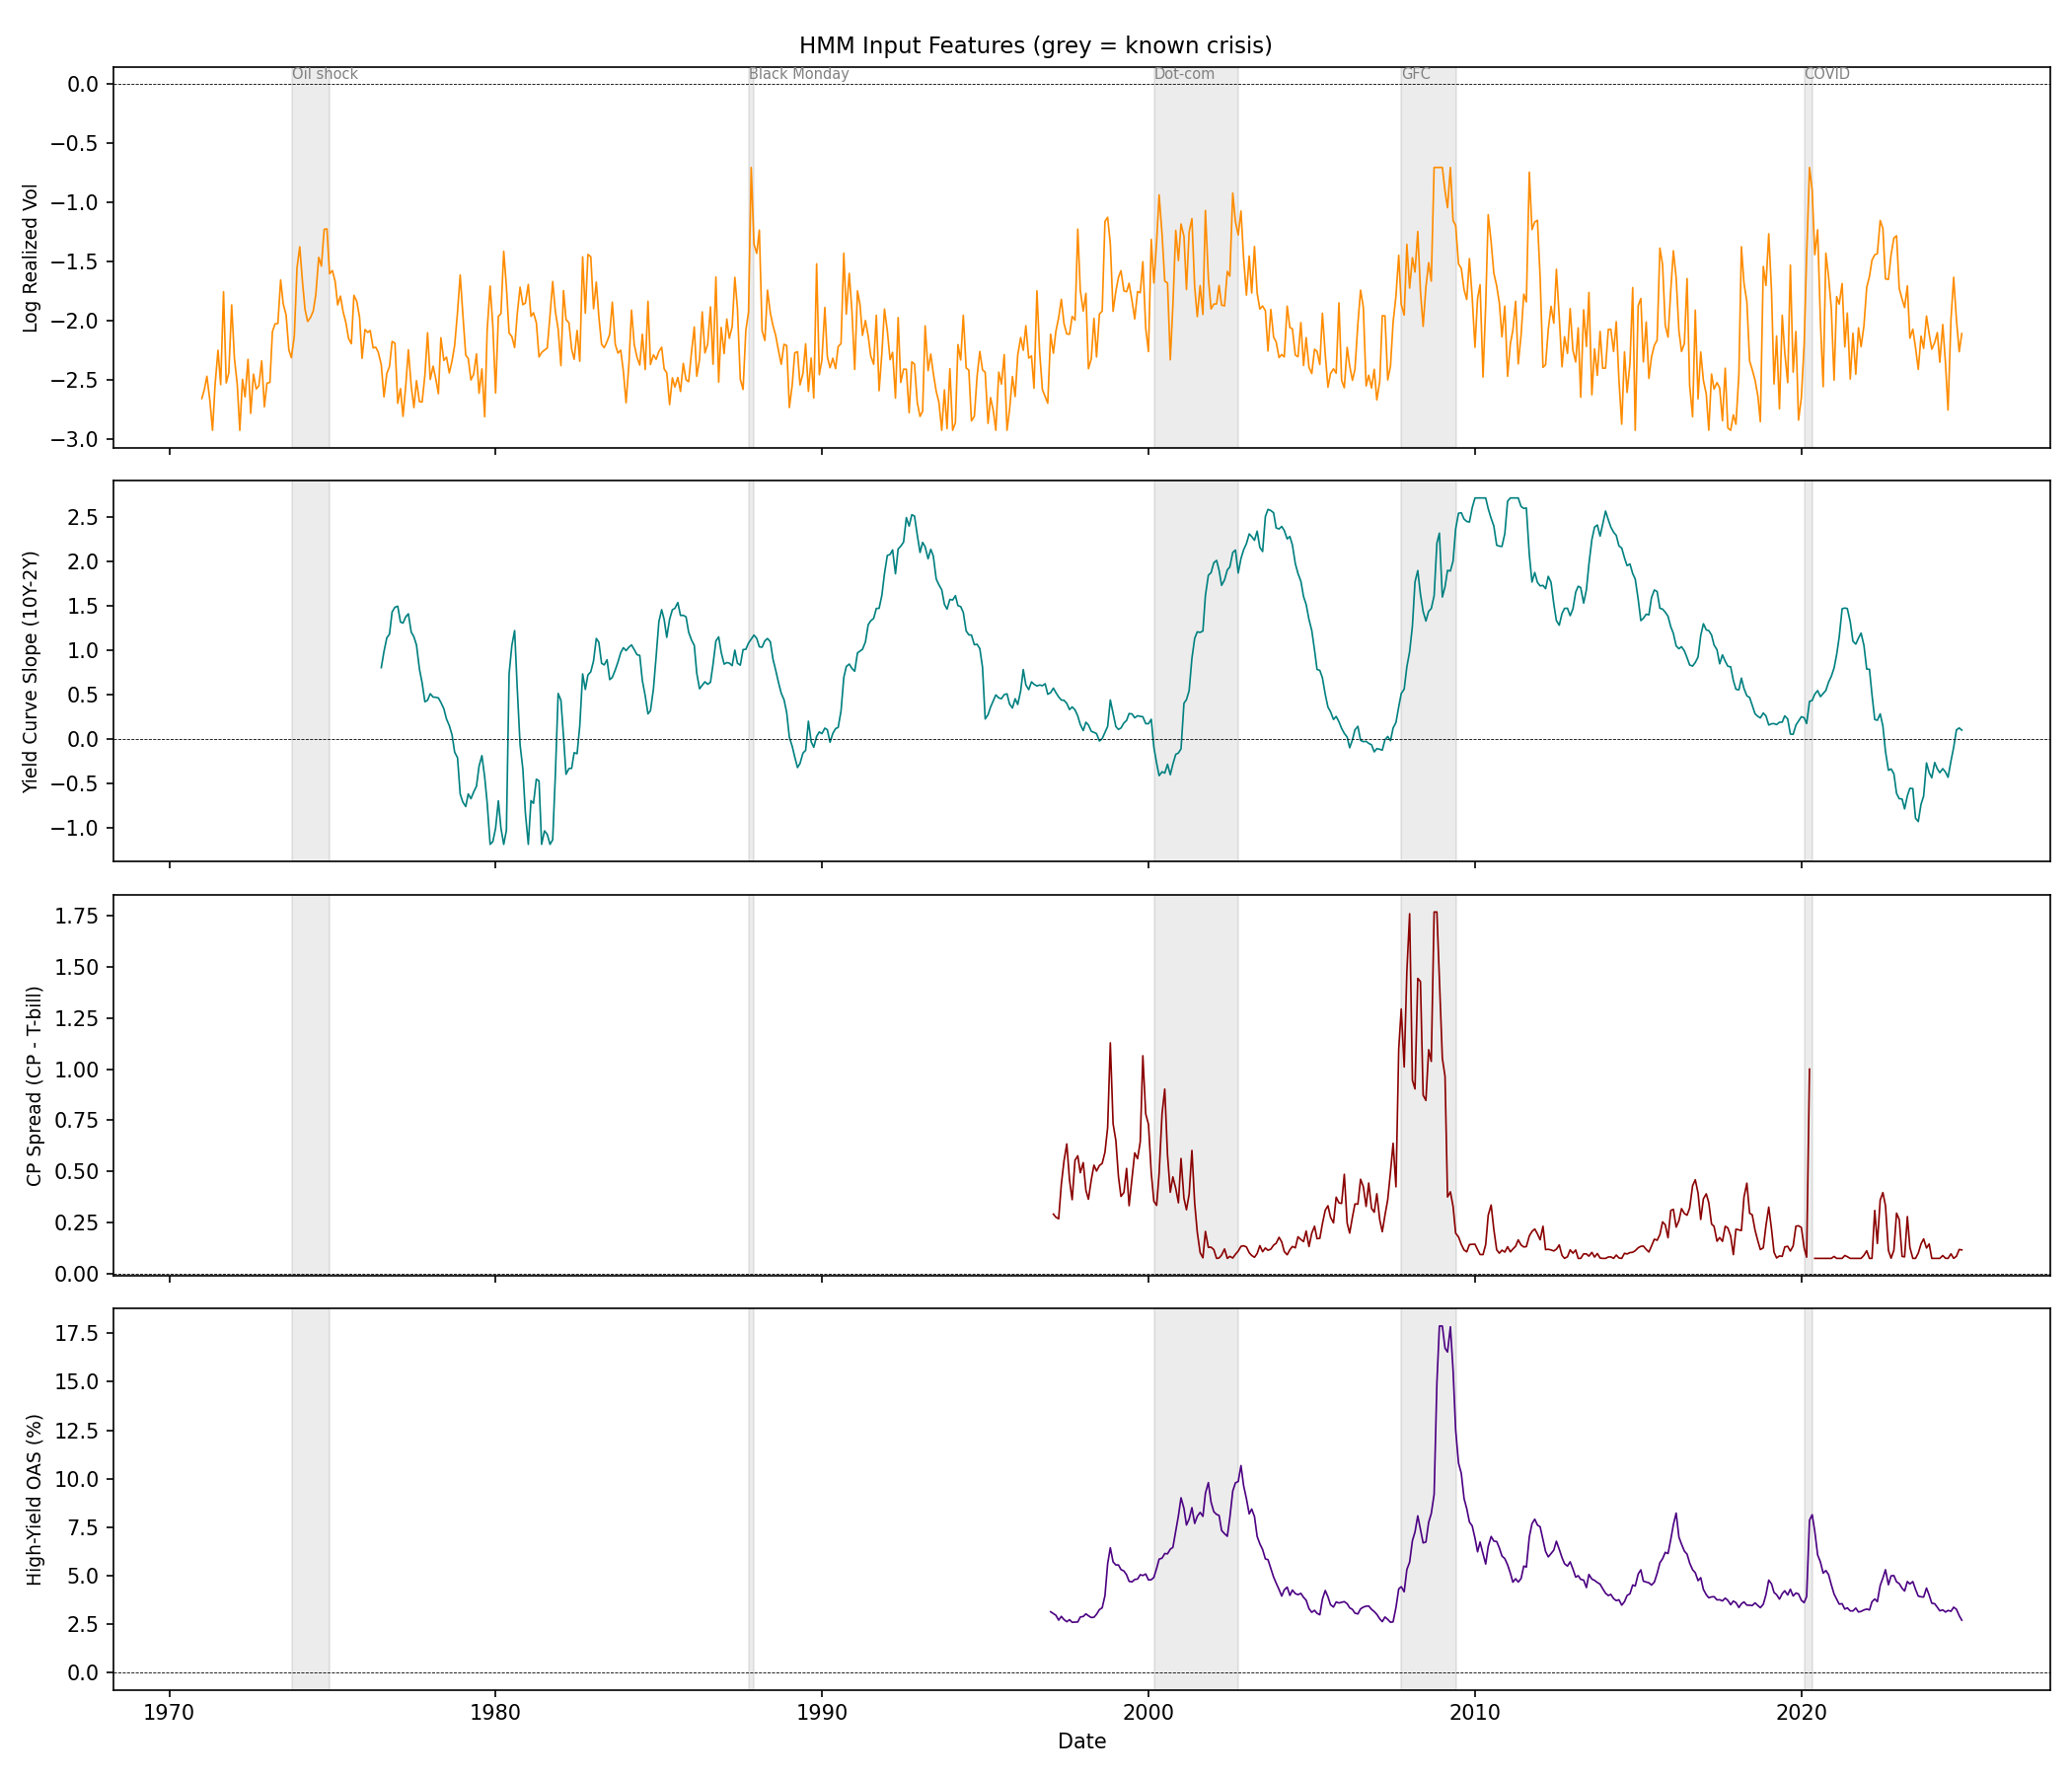
\includegraphics[width=\textwidth]{features_hmm.png}
    \caption{Time series of the four HMM input features (DD, DISP, REL\_N, CS), standardised using training-sample statistics. Shaded regions indicate NBER recession periods. All four features respond during the dot-com bust (2000--2002) and the global financial crisis (2007--2009), but with distinct dynamics reflecting their complementary stress dimensions.}
    \label{fig:features_hmm}
\end{figure}

\paragraph{Why these four features together}
The four selected indicators span complementary dimensions of market stress: DD captures the depth of equity market declines, DISP and REL\_N describe cross-sectional behaviour (stock disagreement and structural attrition), and CS captures corporate credit conditions. The feature selection procedure in Section~\ref{sec:feature_selection} confirms that this combination, drawn from a broader candidate pool of nine indicators including volatility and options market indicators, produces the most robust regime signal for the downstream momentum strategies.

\paragraph{Preprocessing}
All four features are winsorised at the 1st and 99th percentiles to limit the influence of extreme outliers.\footnote{Winsorisation replaces observations below the $p$-th percentile with the $p$-th percentile value, and observations above the $(1-p)$-th percentile with the $(1-p)$-th percentile value. Unlike trimming, which discards extreme observations entirely, winsorisation retains all data points while bounding their magnitude. This is particularly important for the HMM emission densities, which assume multivariate normality and can be distorted by heavy-tailed outliers.} The winsorisation bounds are computed on the training sample (1990--2010) and applied unchanged to the test sample, preventing information leakage. After winsorisation, each feature is standardised to zero mean and unit variance using training-sample statistics:
\begin{equation}
    z_{j,t} = \frac{x_{j,t} - \bar{x}_j^{\text{train}}}{\sigma_j^{\text{train}}}.
\end{equation}
Standardisation ensures that all features contribute equally to the HMM's Gaussian emission densities, so that the regime classification is not dominated by whichever feature has the largest raw scale.

\subsection{HMM Feature Selection}\label{sec:feature_selection}

The choice of HMM input features has a substantial impact on regime classification quality and, ultimately, on portfolio performance. This thesis selects features through a systematic three-pass pipeline that progressively filters candidates and increases computational rigor at each stage.

\paragraph{Candidate pool}
Nine monthly macrofinancial indicators, all available from 1990 onward, are considered as HMM inputs. These span three broad categories of market stress:
\begin{itemize}
    \item \emph{Equity market:} market drawdown (DD), realised volatility (VOL), cross-sectional return dispersion (DISP), relative market participation (REL\_N), advance-decline ratio (ADR), and cross-sectional return skewness (SKEW).
    \item \emph{Credit and macro:} BAA--AAA credit spread (CS), log VIX (LVIX), and the 10-year minus 2-year Treasury term spread (TERM).
\end{itemize}
All candidates are observable in real time at the end of each month. Two additional credit indicators (the commercial paper spread and the high-yield option-adjusted spread) are excluded because their data begins in the mid-1990s, providing insufficient training coverage for the 1990--2010 estimation window. All features are standardised to $z$-scores using training-period means and standard deviations, applied unchanged to the test period.

\paragraph{Pass~1: Quality screen}
Because market drawdown (DD) is the most economically direct measure of equity stress and consistently emerges as the dominant regime-identifying feature, it is required in every combination. The remaining eight candidates are combined with DD in groups of 1 to 3 additional features, yielding $1 + \binom{8}{1} + \binom{8}{2} + \binom{8}{3} = 93$ combinations spanning 1- to 4-feature HMMs. Each combination is estimated with a single Gibbs sampler seed (2{,}000 iterations, 500 burn-in). A combination passes the quality screen if it satisfies five criteria: (i)~minimum effective sample size (ESS) across all posterior mean parameters exceeds 50; (ii)~at least $\min(2, D)$ features exhibit statistically significant regime separation (95\% credible interval excluding zero); (iii)~the average filtered panic probability during the GFC (October 2007 to June 2009) exceeds 0.5 and during COVID (February to May 2020) exceeds 0.5; (iv)~the average panic probability during non-crisis reference periods (January 2003 to December 2006, and January 2013 to December 2019) remains below 0.4; and (v)~the Dot-com crash (March 2000 to October 2002) average exceeds 0.3. Panic state identification uses the same sign-correction method as the main HMM (Section~\ref{sec:gibbs}): the direction of each feature during known crises is determined empirically, and the state with the higher sign-corrected posterior mean is labelled as panic.

\paragraph{Pass~2: Portfolio ranking}
Surviving combinations are evaluated through the full cross-sectional pipeline. The filtered probability $\pi_t^{\text{filter}}$ is averaged across 5 HMM seeds to reduce MCMC noise. XGBoost predictions are averaged across 10 seeds to stabilise stock rankings. To maintain a fair comparison with the exposure-scaling approach of \citet{DanielMoskowitz2016}, portfolios use momentum and $\pi_t^{\text{filter}}$ only (no fundamental features) and are constructed as long-short with 10 basis points one-way costs applied to both legs. Combinations are ranked by out-of-sample Sharpe ratio. The top 10 advance to Pass~3.

\paragraph{Pass~3: Definitive validation}
The final pass increases seed counts to 10 HMM seeds and 20 XGBoost seeds. For each surviving combination, four tests are conducted:
\begin{enumerate}
    \item \emph{Ensemble Sharpe ratio} from the averaged predictions, representing the strategy's performance under heavy seed averaging.
    \item \emph{Sub-period consistency}: Sharpe ratios for 2011--2015, 2016--2020, and 2021--2025, verifying that performance is not driven by a single sub-period.
    \item \emph{Stability test}: 20 independent experiments, each using a random partition of 3 HMM seeds and 1 XGBoost seed drawn from a pool of 20, to assess sensitivity to the specific seed combination. Combinations are classified as stable ($\sigma < 0.10$), moderate ($0.10 \leq \sigma < 0.15$), or unstable ($\sigma \geq 0.15$).
    \item \emph{Leave-one-year-out}: each test-period year is dropped in turn to verify that no single year drives the result.
\end{enumerate}

\paragraph{Feature count comparison}
The pipeline evaluates combinations of 1 to 4 features to determine the optimal model complexity. Table~\ref{tab:feature_selection} reports the top combination at each feature count. Four features (DD+DISP+REL\_N+CS) achieves the highest stability mean (0.804) with the lowest standard deviation (0.082), indicating that the additional features reduce seed sensitivity without introducing overfitting. This combination is confirmed by a heavy variance test: 10 independent runs, each using 20 fresh HMM seeds (seeds 1--200) and 50 XGBoost seeds, produce a mean Sharpe of 0.804 with standard deviation 0.082.

\begin{table}[H]
\centering
\small
\begin{tabular}{c l r r r}
\toprule
$D$ & Combination & Sharpe & Mean & $\sigma$ \\
\midrule
4 & DD+DISP+REL\_N+CS & 0.91 & 0.84 & 0.11 \\
4 & DD+DISP+CS+TERM & 0.82 & 0.55 & 0.15 \\
4 & DD+DISP+REL\_N+SKEW & 0.80 & 0.69 & 0.08 \\
4 & DD+VOL+DISP+REL\_N & 0.80 & 0.77 & 0.09 \\
3 & DD+DISP+REL\_N & 0.77 & 0.77 & 0.10 \\
4 & DD+VOL+DISP+TERM & 0.71 & 0.67 & 0.16 \\
3 & DD+VOL+CS & 0.69 & 0.43 & 0.13 \\
1 & DD & 0.68 & 0.67 & 0.14 \\
4 & DD+DISP+REL\_N+TERM & 0.62 & 0.45 & 0.18 \\
3 & DD+ADR+TERM & 0.57 & 0.69 & 0.07 \\
\bottomrule
\end{tabular}
\caption{Top 10 feature combinations from the three-pass selection pipeline (long-short, 10 bps costs). $D$ = number of HMM features. Sharpe = ensemble Sharpe ratio (10 HMM seeds, 20 XGBoost seeds). Mean and $\sigma$ are the mean and standard deviation of the Sharpe ratio across 5 independent experiments with different seed partitions, measuring robustness to random initialisation. DD+DISP+REL\_N+CS ranks first on both ensemble Sharpe and stability mean.}
\label{tab:feature_selection}
\end{table}


\paragraph{Ablation analysis}
Single-feature and leave-one-out experiments isolate each feature's marginal contribution to the selected combination. DD alone achieves a Sharpe of 0.66, confirming its role as the dominant stress indicator. In the leave-one-out analysis, removing DD or REL\_N causes the largest performance drops ($-0.46$ and $-0.54$, respectively), while DISP and CS each contribute less than 0.01 marginally. Despite their small marginal contributions, DISP and CS improve the stability of the regime signal by providing independent information from different market segments (cross-sectional disagreement and corporate credit stress, respectively). The full ablation results are reported in Section~\ref{sec:ablation_results}.

\paragraph{Summary}
The selected feature set, DD+DISP+REL\_N+CS, captures market stress through three complementary dimensions: the depth of equity market declines (DD), cross-sectional stock disagreement (DISP) and structural market attrition (REL\_N), and corporate credit conditions (CS). All four features are available from January 1990, providing 241 training months that include both the dot-com crash and the global financial crisis. The final $\pi_t^{\text{filter}}$ used in all subsequent analyses is averaged across 200 HMM seeds and passes all three validation checks (regime separation, crisis alignment, and MCMC convergence).

\subsection{Cross-Sectional Features}\label{sec:cs_features}

The cross-sectional models use three groups of features to rank stocks each month: momentum signals, the filtered panic probability $\pi_t^{\text{filter}}$, and fundamental characteristics.

\paragraph{Momentum lookbacks}
Twelve trailing momentum signals are computed for each stock, corresponding to lookback horizons of 1 to 12 months:
\begin{equation}
    \text{mom}_{k,t}^s = \prod_{\ell=1}^{k}(1 + r_{t-\ell}^s) - 1, \qquad k = 1, \dots, 12,
\end{equation}
where $r_{t-\ell}^s$ is the adjusted return of stock $s$ in month $t - \ell$. Note that the current month's return is excluded from all lookbacks to avoid mechanical correlation with the forward return being predicted. Including all twelve horizons rather than a single lookback (e.g., the standard 12-month momentum of \citet{JegadeeshTitman1993}) allows the models to learn which horizons are most informative in each regime. As shown in Section~\ref{sec:ic_analysis}, intermediate-term lookbacks (8--11 months) dominate in calm markets, while 1-month momentum becomes important during panic due to short-term reversal dynamics.

\paragraph{Regime signal}
The filtered panic probability $\pi_t^{\text{filter}}$ from the HMM enters as a single feature. Because it varies only at the monthly market level (every stock in the same month receives the same value), it functions as a conditioning variable rather than a stock-level predictor. Its role in the cross-sectional models is discussed in Section~\ref{sec:ic_analysis}.

\paragraph{Fundamental characteristics}
Seven firm-level characteristics are computed from Compustat quarterly data. These variables are drawn from the established asset pricing literature: book-to-market and size are the original \citet{FamaFrench2015} factors, gross profitability follows \citet{NovyMarx2013}, and the remaining variables (leverage, asset growth, return on equity, earnings growth) capture investment and quality dimensions that have been shown to predict cross-sectional returns. Their role in the models is not to generate additional returns but to act as a quality screen that compresses portfolio volatility (see Section~\ref{sec:performance_results}).

\begin{itemize}
    \item \textbf{Book-to-market (bm):} Book equity divided by market equity, $\text{ceqq} / ME$. Captures the value premium.
    \item \textbf{Return on equity (roe):} Income before extraordinary items divided by book equity, $\text{ibq} / \text{ceqq}$. Measures profitability.
    \item \textbf{Gross profitability:} Revenue minus cost of goods sold, scaled by total assets, $(\text{revtq} - \text{cogsq}) / \text{atq}$. Follows the profitability factor of \citet{NovyMarx2013}.
    \item \textbf{Asset growth:} Year-over-year growth in total assets, $\text{atq}_t / \text{atq}_{t-4} - 1$. Firms with high asset growth tend to have lower future returns.
    \item \textbf{Leverage:} Total debt divided by total assets, $(\text{dlttq} + \text{dlcq}) / \text{atq}$. Highly leveraged firms are more vulnerable to financial distress.
    \item \textbf{Earnings growth:} Year-over-year growth in earnings, computed as $\text{sign}(g) \cdot \log(1 + |g|)$ where $g = \text{ibq}_t / \text{ibq}_{t-4} - 1$. The signed-log transformation handles the fat-tailed distribution of earnings changes.
    \item \textbf{Log market equity:} The natural logarithm of market capitalisation (price times shares outstanding), lagged one month. Controls for the size effect.
\end{itemize}

Market equity is computed as the absolute value of the end-of-month stock price multiplied by shares outstanding from CRSP. The absolute value handles cases where CRSP reports the bid-ask midpoint as a negative price.

All fundamental variables are lagged by four months relative to the fiscal quarter end to ensure that accounting data would have been publicly available at the time of portfolio formation, consistent with the standard approach in the empirical asset pricing literature. This lag accounts for the SEC filing deadline and prevents look-ahead bias. Each month, the most recent available quarter's fundamentals are assigned to each stock using a backward merge, so that no future accounting information is used. Fundamentals are winsorised at the 1st and 99th percentiles (5th and 95th for asset growth, which has a fatter right tail), with bounds computed on the training sample only.

\paragraph{Missing data handling}
Not all stocks have complete fundamental coverage in every month. Missing rates range from approximately 7\% (return on equity, leverage) to 17\% (gross profitability). For the logistic regression model, which cannot handle missing values, fundamentals are imputed at the training-sample median prior to standardisation. For XGBoost, which natively handles missing values by learning optimal split directions for absent features, no imputation is applied. In both cases, stocks are only excluded if core features (momentum lookbacks or the regime signal) are missing.

\subsection{Train--Test Split and Information Leakage Prevention}\label{sec:split}

The sample is divided at December 2010. The HMM start date of January 1990 is determined by the availability of sufficient stock-level data for computing cross-sectional return dispersion, and the split point is chosen so that the training period contains at least two full market cycles, including the dot-com crash (2000--2002) and the global financial crisis (2007--2009), giving the HMM sufficient exposure to both calm and panic regimes. The training period is used for all model estimation: HMM Gibbs sampling, logistic regression fitting, and XGBoost training. The test period (January 2011 to November 2025, 167 months) is reserved exclusively for out-of-sample evaluation; no model parameters are re-estimated or updated during this period.

Several safeguards prevent information leakage from the test period into model training:
\begin{itemize}
    \item Winsorisation bounds and standardisation statistics (means, standard deviations) are computed on the training sample and applied unchanged to the test sample.
    \item The HMM posterior mean parameters (regime means $\boldsymbol{\mu}_k$, covariances $\boldsymbol{\Sigma}_k$, and transition matrix $\mathbf{P}$) are estimated on the training period and frozen. During the test period, only the forward-filtering recursion is run using the fixed parameters, producing the causal signal $\pi_t^{\text{filter}}$ without any parameter updating.
    \item The cross-sectional models are trained once on the training sample and applied without retraining to the test sample.
    \item NYSE breakpoints for portfolio decile assignment are computed each month using only NYSE-listed stocks in that month, which is observable in real time.
\end{itemize}

A single fixed split is standard in the literature that this thesis builds on \citep[e.g.,][]{GHM2023} and is appropriate given the computational cost of re-estimating the Bayesian HMM via Gibbs sampling. Alternative train/test splits (Appendix~\ref{app:alt_splits}) confirm that both M1 and M2 produce positive Sharpe ratios across all splits tested, though the baseline split yields the strongest M1 performance. The 14-year out-of-sample test period and the statistical significance tests reported in Section~\ref{sec:performance_results} further mitigate concerns about split dependence.
